\chapter{Project Plan}

\section{Organizzazione Complessiva del Project Plan}

La realizzazione di \textit{Tuning Ledger}, la piattaforma per la gestione del \textit{Digital Modified Vehicle Passport} (DMVP), richiede una pianificazione dettagliata e suddivisa in fasi, al fine di garantire un avanzamento efficace del lavoro e un monitoraggio costante dei risultati.

Il Project Plan copre un arco temporale di sei anni ed è articolato in due fasi principali:

\begin{itemize}
    \item \textbf{Prima Fase: progettazione, sviluppo e deployment della piattaforma.}
    \begin{itemize}
        \item \textit{Descrizione}: realizzazione completa del sistema informativo, comprensiva dell'infrastruttura blockchain permissioned, dei micro-servizi applicativi e delle interfacce destinate agli attori della filiera.
        \item \textit{Durata}: 1 anno.
    \end{itemize}
    \item \textbf{Seconda Fase: promozione, esercizio e mantenimento della piattaforma.}
    \begin{itemize}
        \item \textit{Descrizione}: a seguito del rilascio, la piattaforma entra in una fase di espansione commerciale e operativa nel mercato dell'automotive tuning, durante la quale vengono erogate le attività di supporto tecnico, onboarding degli attori, analisi dei dati di esercizio e sviluppo continuo per l'adeguamento normativo.
        \item \textit{Durata}: 5 anni.
    \end{itemize}
\end{itemize}

Le due fasi hanno inizio il 1\textdegree{} gennaio 2026 e termine il 31 dicembre 2031, come riassunto nel diagramma di GANTT complessivo riportato in Figura~\ref{fig:gantt-complessivo}.

\begin{figure}[H]
    \centering
    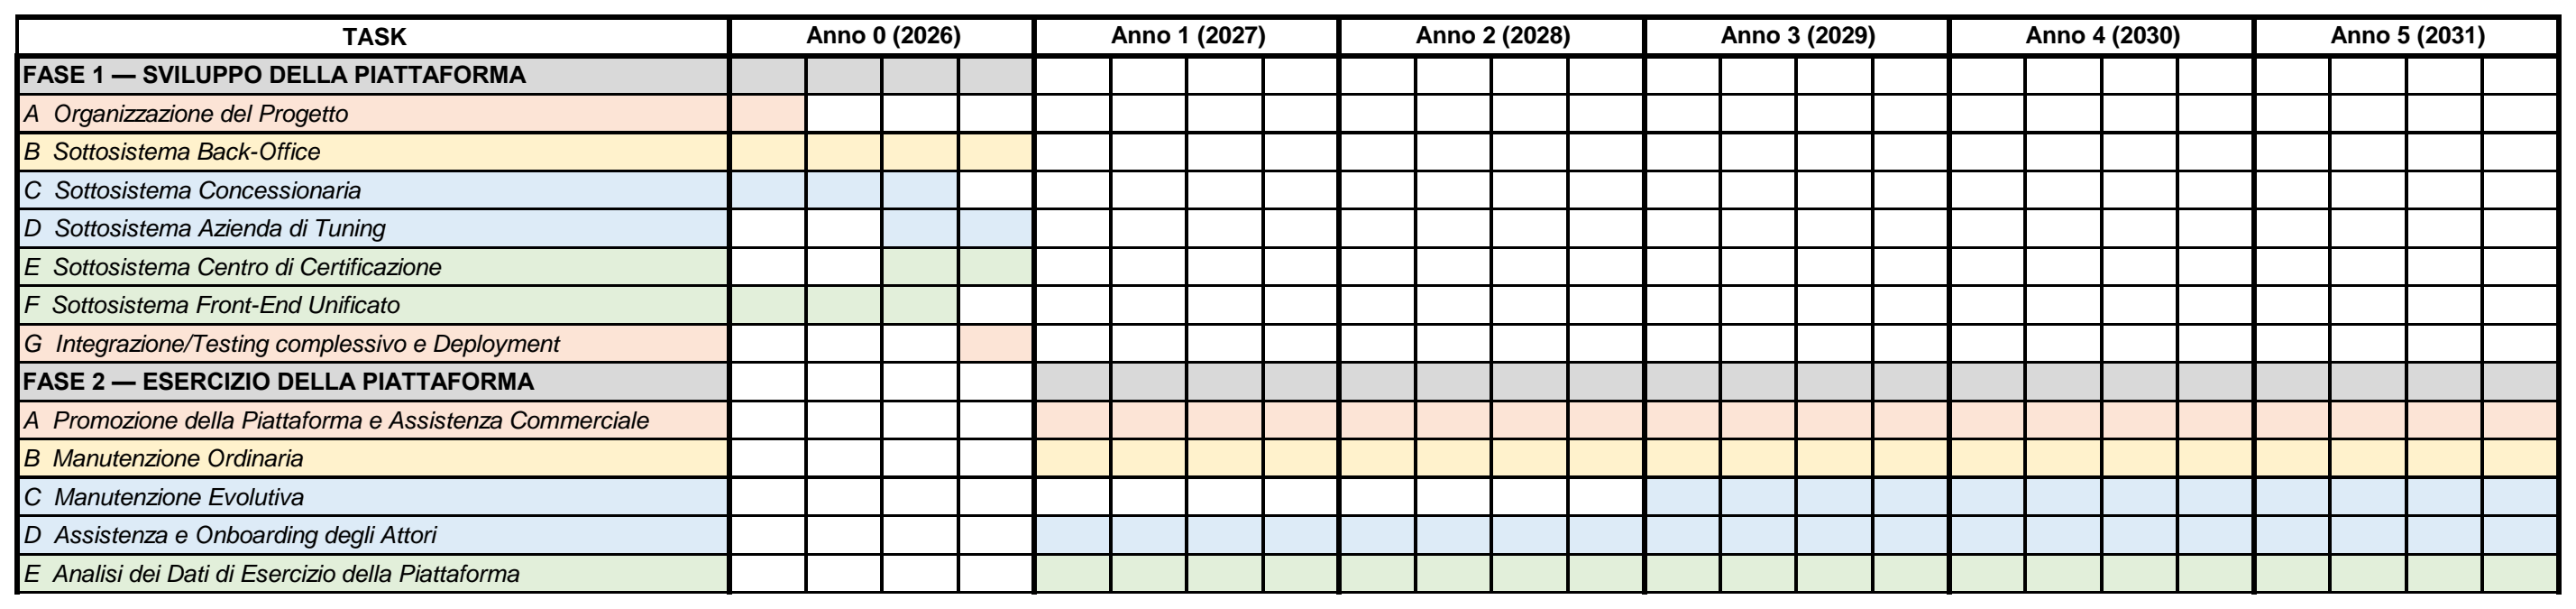
\includegraphics[width=\textwidth]{imgs/gantt/gantt_complessivo.png}
    \caption{Diagramma di GANTT complessivo del progetto}
    \label{fig:gantt-complessivo}
\end{figure}

Le figure professionali impiegate nel progetto, necessarie a garantire la corretta esecuzione delle attività, sono le seguenti:

\begin{itemize}
    \item \textbf{Project Manager (PM)}: si occupa della pianificazione, della gestione e del coordinamento dell'intero progetto, supervisionando le attività di sviluppo, l'allineamento ai requisiti individuati nella modellazione degli use case, il rapporto con gli stakeholder della filiera e il monitoraggio del budget.
    \item \textbf{Software Architect (SA)}: si occupa della progettazione e della definizione dell'architettura a micro-servizi e dell'infrastruttura blockchain, definendo la logica del \textit{chaincode}, le politiche di \textit{endorsement} della rete permissioned e la separazione tra dati on-chain e off-chain.
    \item \textbf{Full Stack Developer (FSD)}: si occupa dello sviluppo completo del software, gestendo sia le interfacce web e mobile destinate agli attori, sia le logiche di back-end e l'interazione con il \textit{chaincode}; assicura inoltre la guida tecnica dei gruppi di lavoro.
    \item \textbf{Full Stack Developer Junior (FSDJ)}: si occupa dello sviluppo dei moduli applicativi di supporto e delle attività di test, lavorando in affiancamento ai Full Stack Developer.
\end{itemize}

Infine, per il progetto si considera che il numero totale di ore di un Anno/Persona (A/P) sia di \textbf{1.752 ore}, equivalenti a 219 giornate lavorative di 8 ore ciascuna. Per semplificare, si assume che le Ore/Persona (O/P) siano distribuite uniformemente nell'arco dell'anno: un Mese/Persona corrisponde quindi a 146 ore e una settimana a 36,5 ore; uno Sprint, della durata di due settimane, equivale pertanto a 73 ore.

\section{Architettura a Componenti della Piattaforma}

L'architettura della piattaforma è ingegnerizzata secondo un modello a \textbf{micro-servizi}, scelta orientata a garantire elevati standard di scalabilità, modularità e manutenibilità del sistema. Tale approccio consente di disaccoppiare le funzionalità di business in componenti software autonomi e indipendenti, ciascuno deputato all'esecuzione di compiti specifici, ottimizzando i cicli di sviluppo e permettendo una scalabilità mirata delle singole risorse.

Al fine di formalizzare la struttura di tale ecosistema tecnologico, la descrizione si avvale di due viste modellistiche basate sullo standard UML (\textit{Unified Modeling Language}):

\begin{itemize}
    \item \textbf{Diagramma dei Componenti}: rappresenta i macro-moduli funzionali, i servizi interni della piattaforma e le relative interfacce di interazione e cooperazione.
    \item \textbf{Diagramma di Distribuzione}: rappresenta la collocazione fisica dei componenti sui nodi di elaborazione e i protocolli di comunicazione impiegati.
\end{itemize}

La Figura~\ref{fig:architettura} illustra la scomposizione logica e i flussi di integrazione dell'architettura complessiva.

\begin{figure}[H]
    \centering
    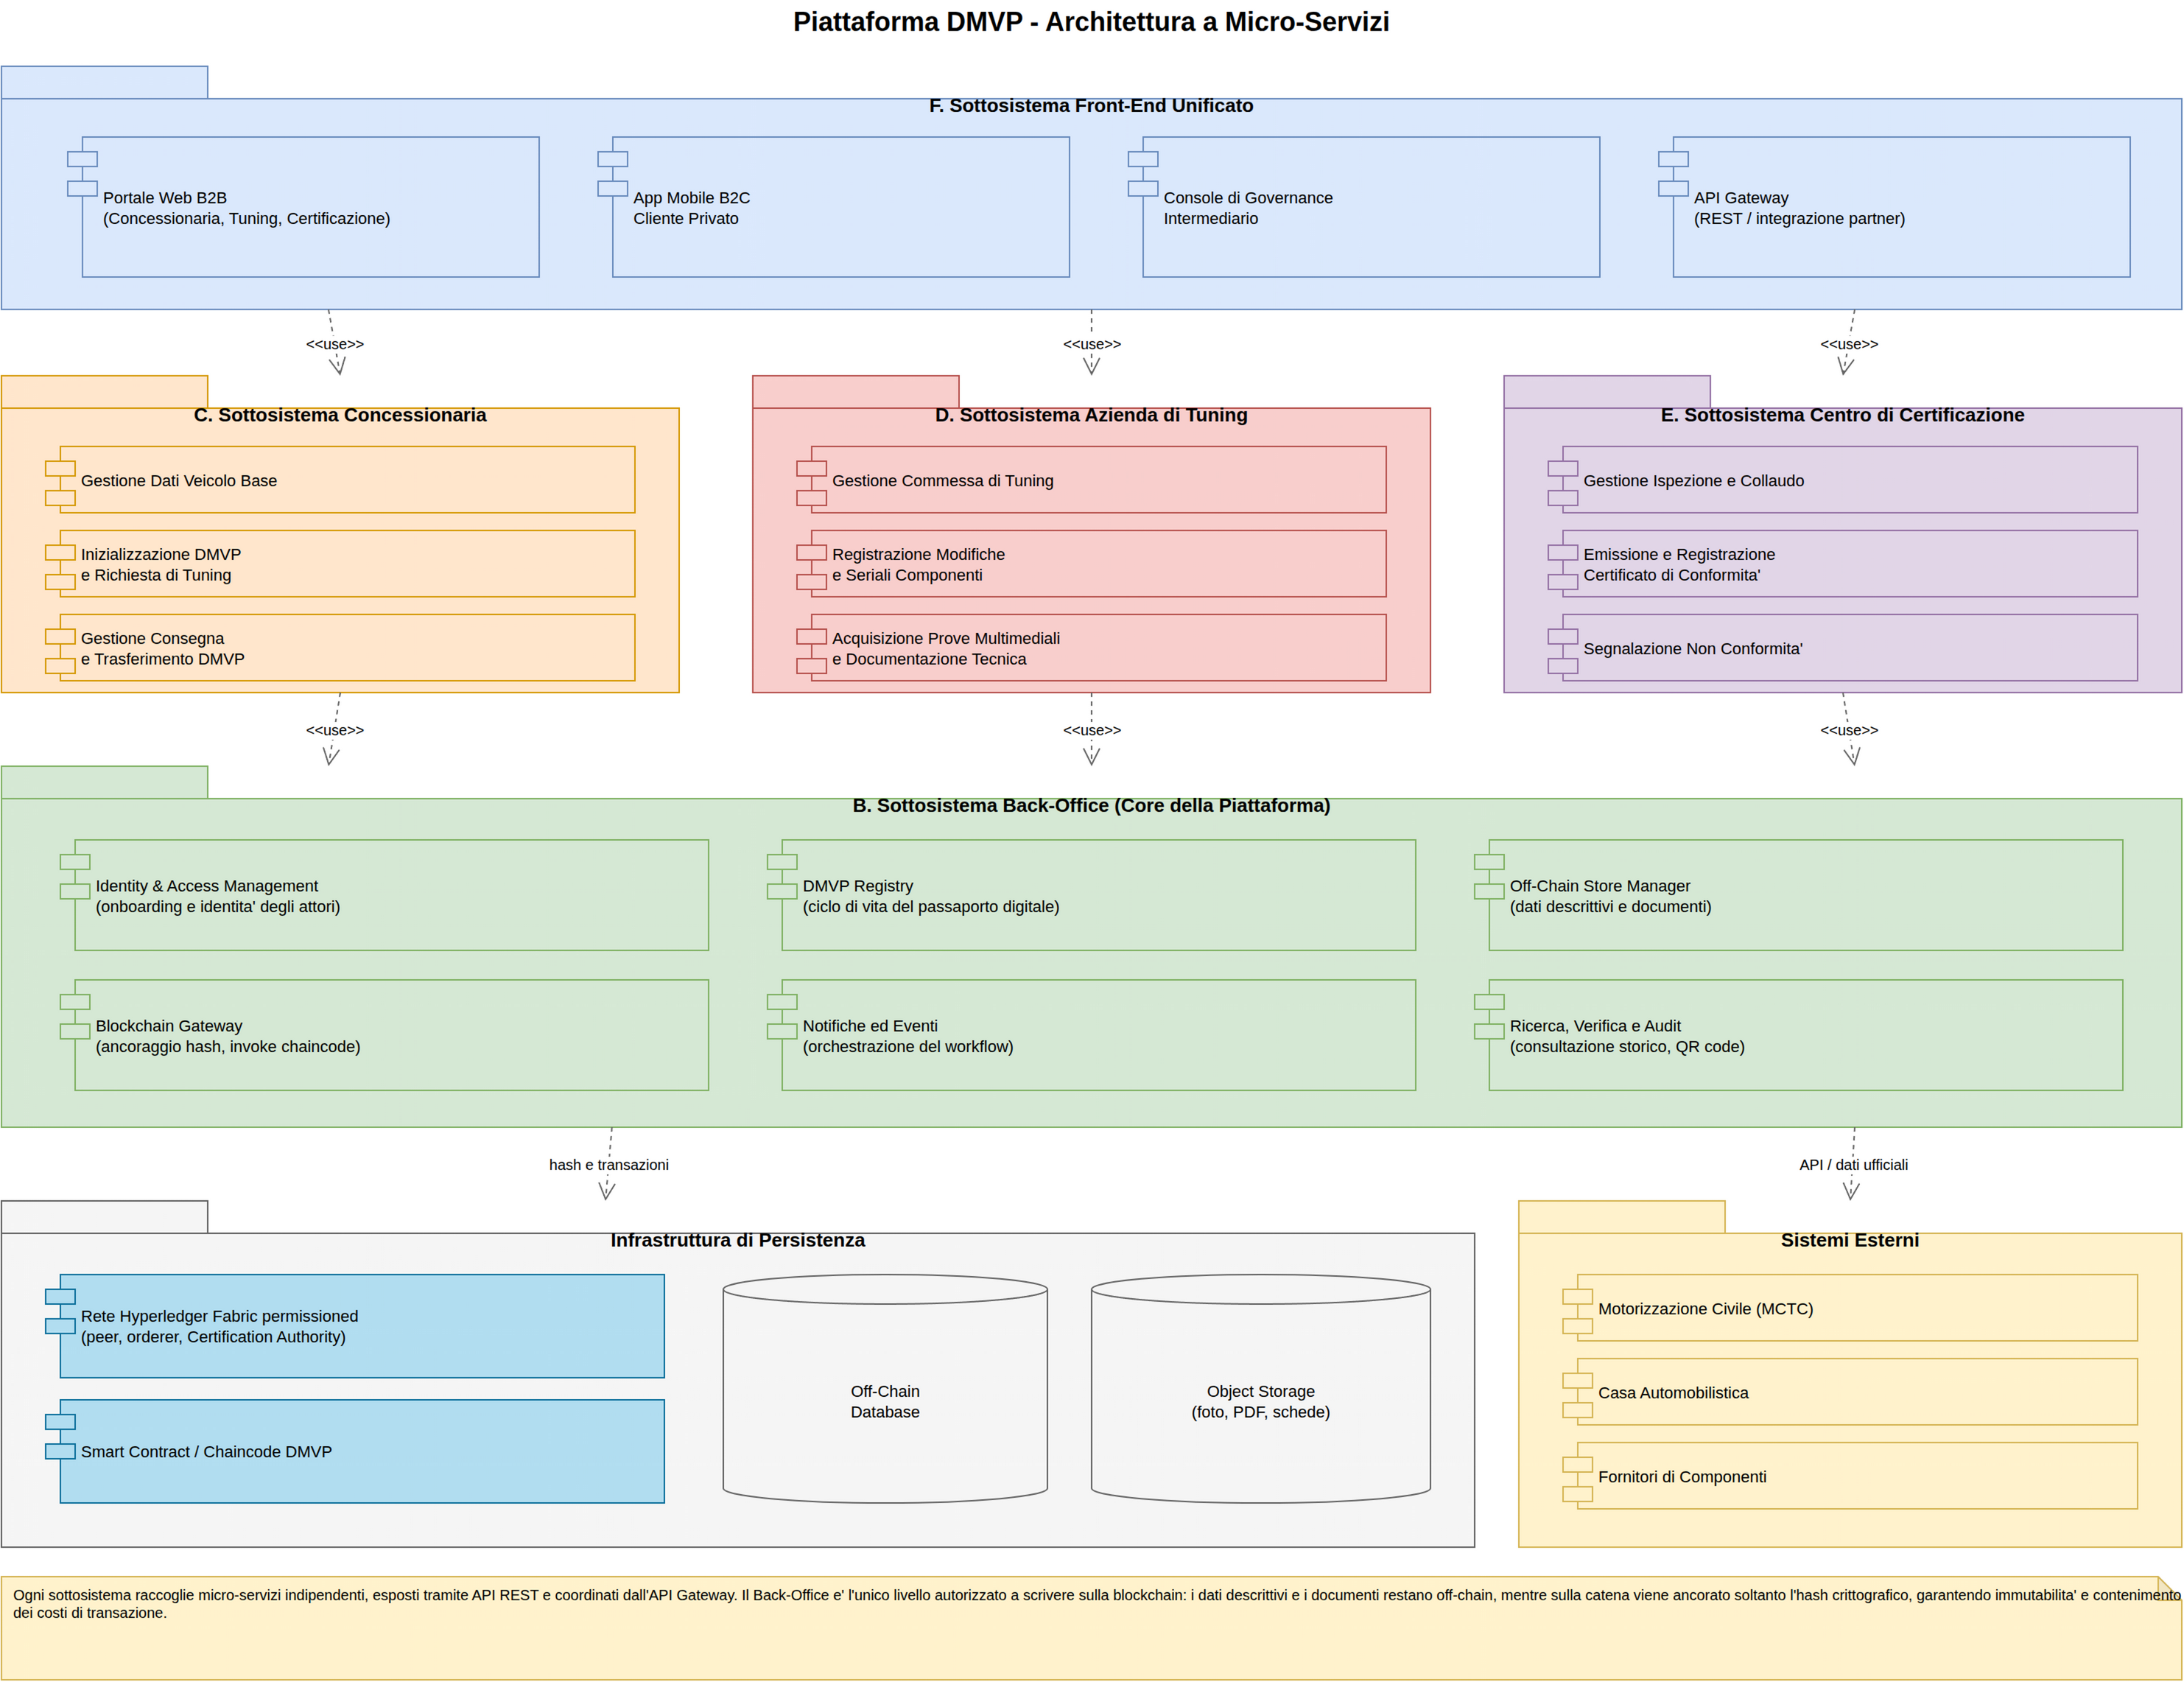
\includegraphics[width=\textwidth]{imgs/projectplan/01_architettura_generale.png}
    \caption{Architettura a micro-servizi della piattaforma DMVP}
    \label{fig:architettura}
\end{figure}

Come si osserva, l'architettura comprende cinque sottosistemi applicativi, poggiati su un'infrastruttura di persistenza ibrida e interfacciati con i sistemi dei partner esterni.

\subsection*{Sottosistema Back-Office}

Il sottosistema Back-Office (Figura~\ref{fig:sub-backoffice}) costituisce il nucleo della piattaforma: comprende tutti i moduli e le logiche computazionali centrali utilizzati in modo trasparente dagli attori, al fine di orchestrare i flussi operativi, gestire la persistenza dei documenti e invocare i metodi esposti dal \textit{chaincode}. Si tratta dell'unico livello autorizzato a scrivere sulla blockchain.

\begin{figure}[H]
    \centering
    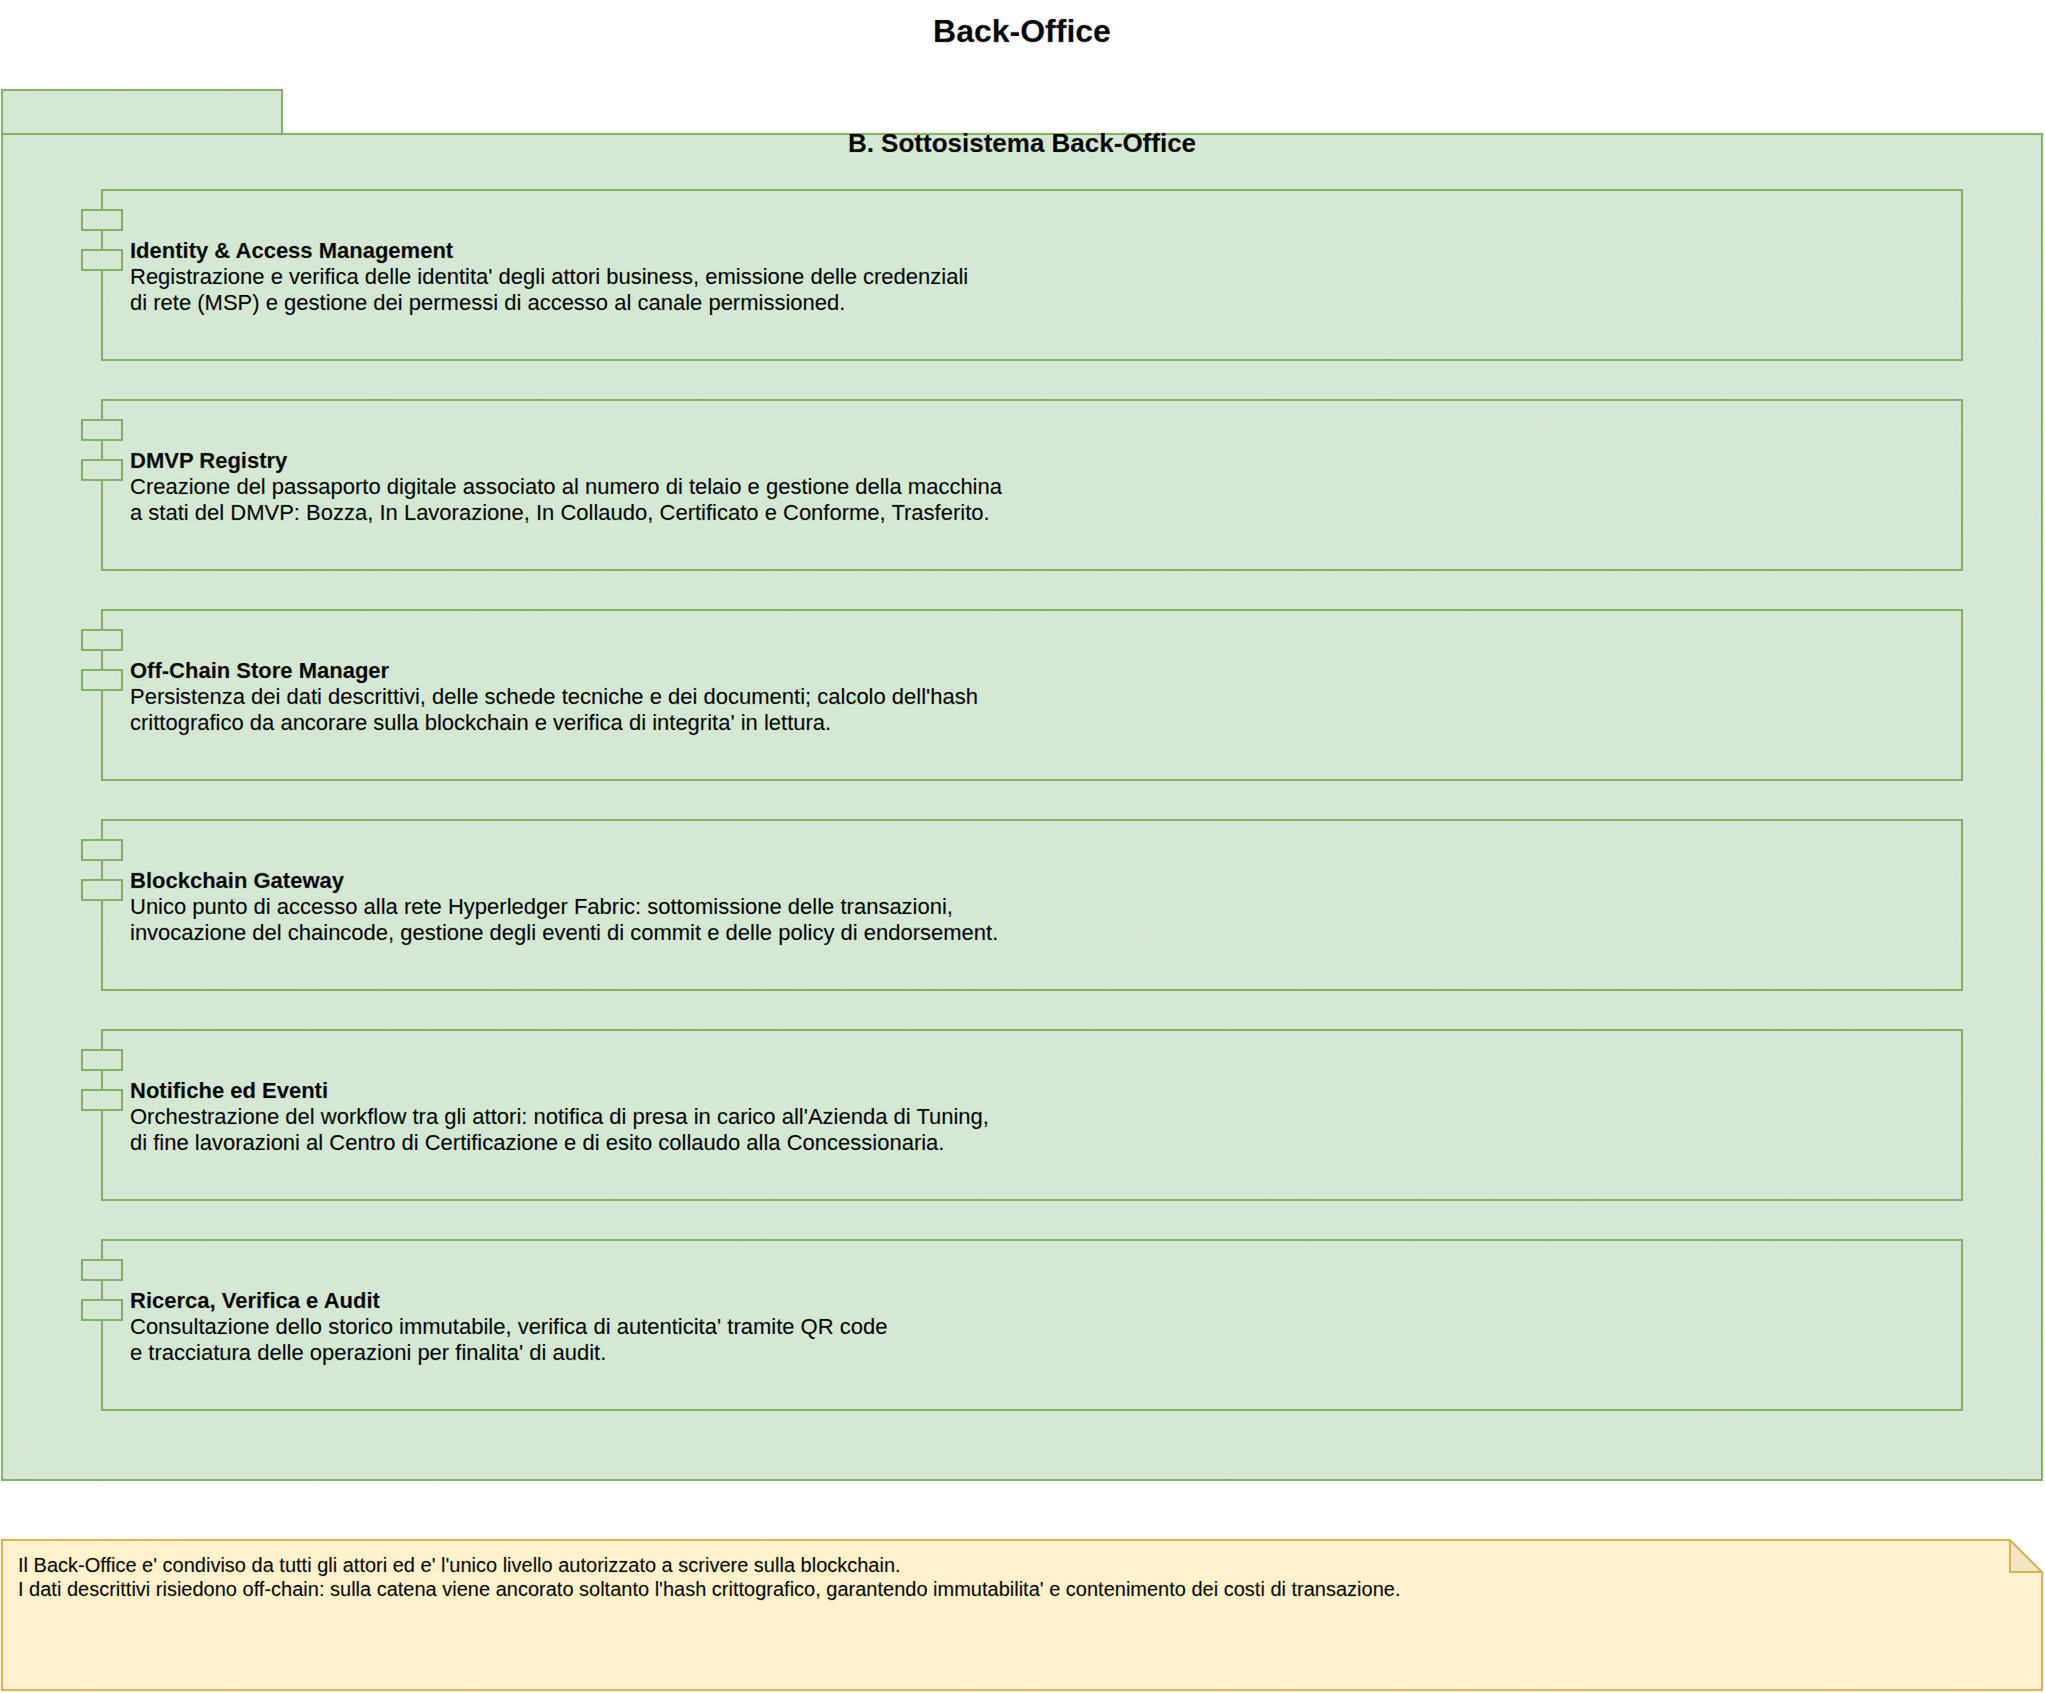
\includegraphics[width=\textwidth]{imgs/projectplan/02_sottosistema_back_office.png}
    \caption{Sottosistema Back-Office}
    \label{fig:sub-backoffice}
\end{figure}

\subsection*{Sottosistema Concessionaria}

Il sottosistema (Figura~\ref{fig:sub-concessionaria}) comprende i moduli dedicati alla Concessionaria, che consentono l'acquisizione e la validazione dei dati identificativi del veicolo originale forniti dalla Casa Automobilistica, la creazione dell'istanza di DMVP e la registrazione delle modifiche commissionate, nonché la gestione della consegna del veicolo omologato e del trasferimento della proprietà del passaporto digitale al Cliente Privato.

\begin{figure}[H]
    \centering
    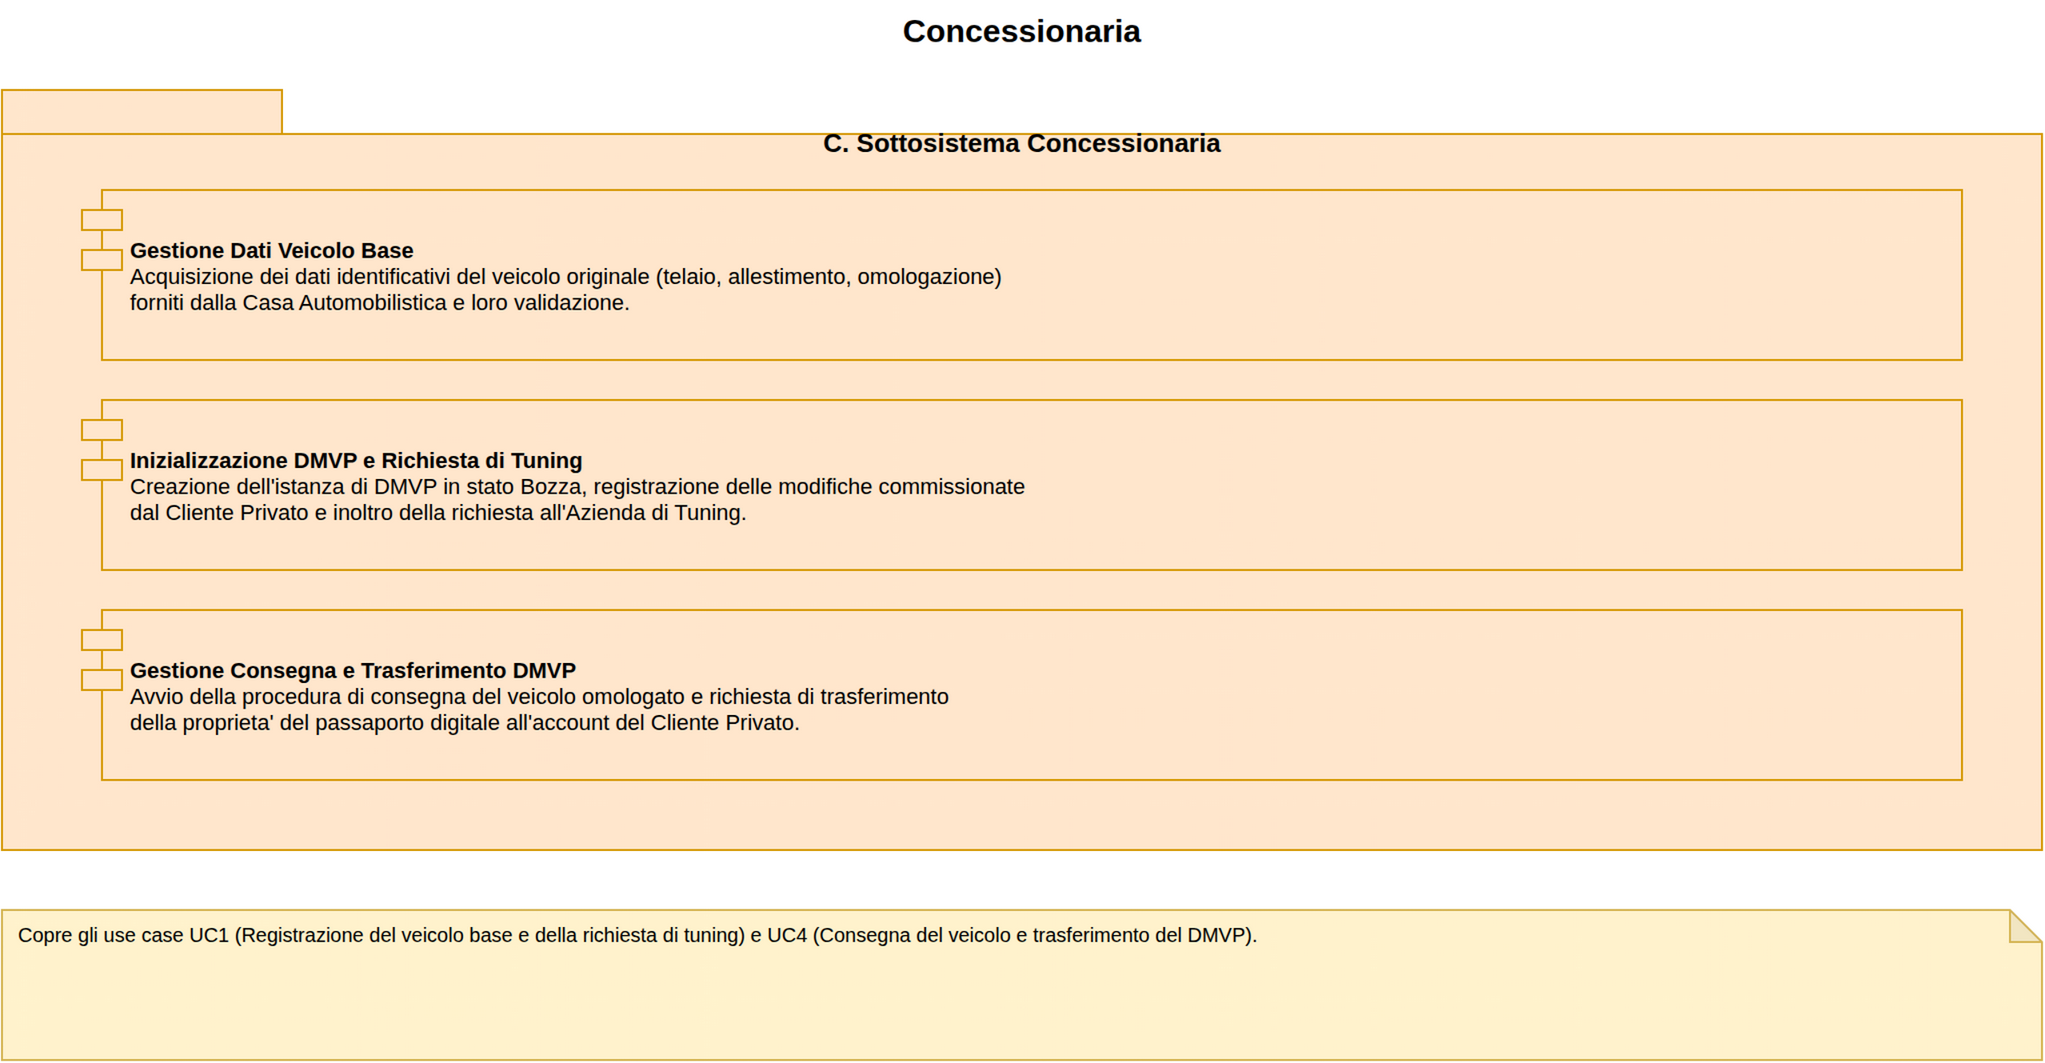
\includegraphics[width=\textwidth]{imgs/projectplan/03_sottosistema_concessionaria.png}
    \caption{Sottosistema Concessionaria}
    \label{fig:sub-concessionaria}
\end{figure}

\subsection*{Sottosistema Azienda di Tuning}

Il sottosistema (Figura~\ref{fig:sub-tuning}) comprende i moduli e le interfacce operative che consentono all'Azienda di Tuning di prendere in carico la commessa, inserire le specifiche tecniche degli interventi e i codici seriali dei componenti installati, e caricare la documentazione tecnica e le prove multimediali a corredo delle lavorazioni eseguite. Rappresenta il cuore operativo della piattaforma, in cui il DMVP viene arricchito in modo immutabile.

\begin{figure}[H]
    \centering
    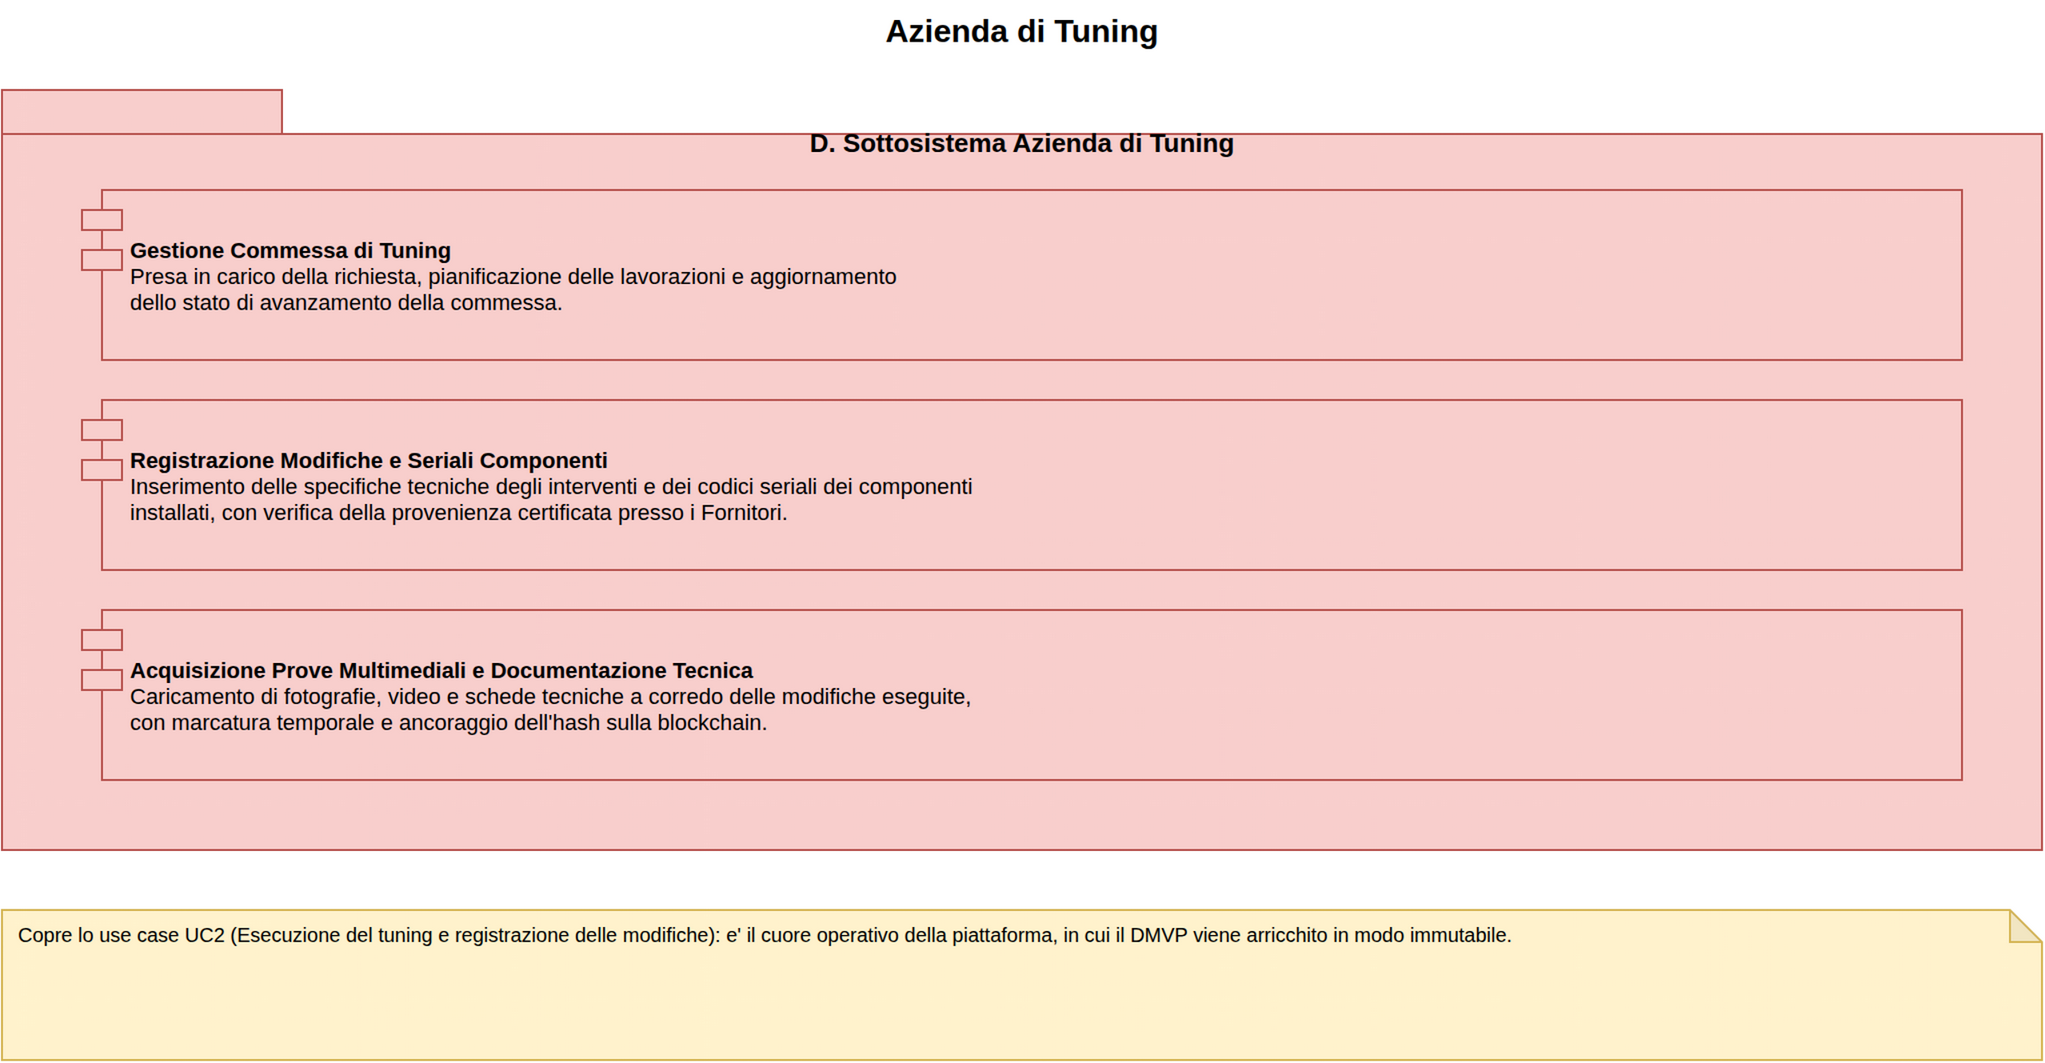
\includegraphics[width=\textwidth]{imgs/projectplan/04_sottosistema_azienda_tuning.png}
    \caption{Sottosistema Azienda di Tuning}
    \label{fig:sub-tuning}
\end{figure}

\subsection*{Sottosistema Centro di Certificazione}

Il sottosistema (Figura~\ref{fig:sub-certificazione}) comprende i moduli destinati al Centro di Certificazione, che permettono la consultazione dello storico immutabile del DMVP, l'esecuzione della checklist normativa e la registrazione degli esiti delle verifiche tecniche, la generazione del certificato digitale firmato con il relativo ancoraggio sulla blockchain e, in caso di esito negativo, la produzione del report di anomalia con reindirizzamento della pratica all'Azienda di Tuning.

\begin{figure}[H]
    \centering
    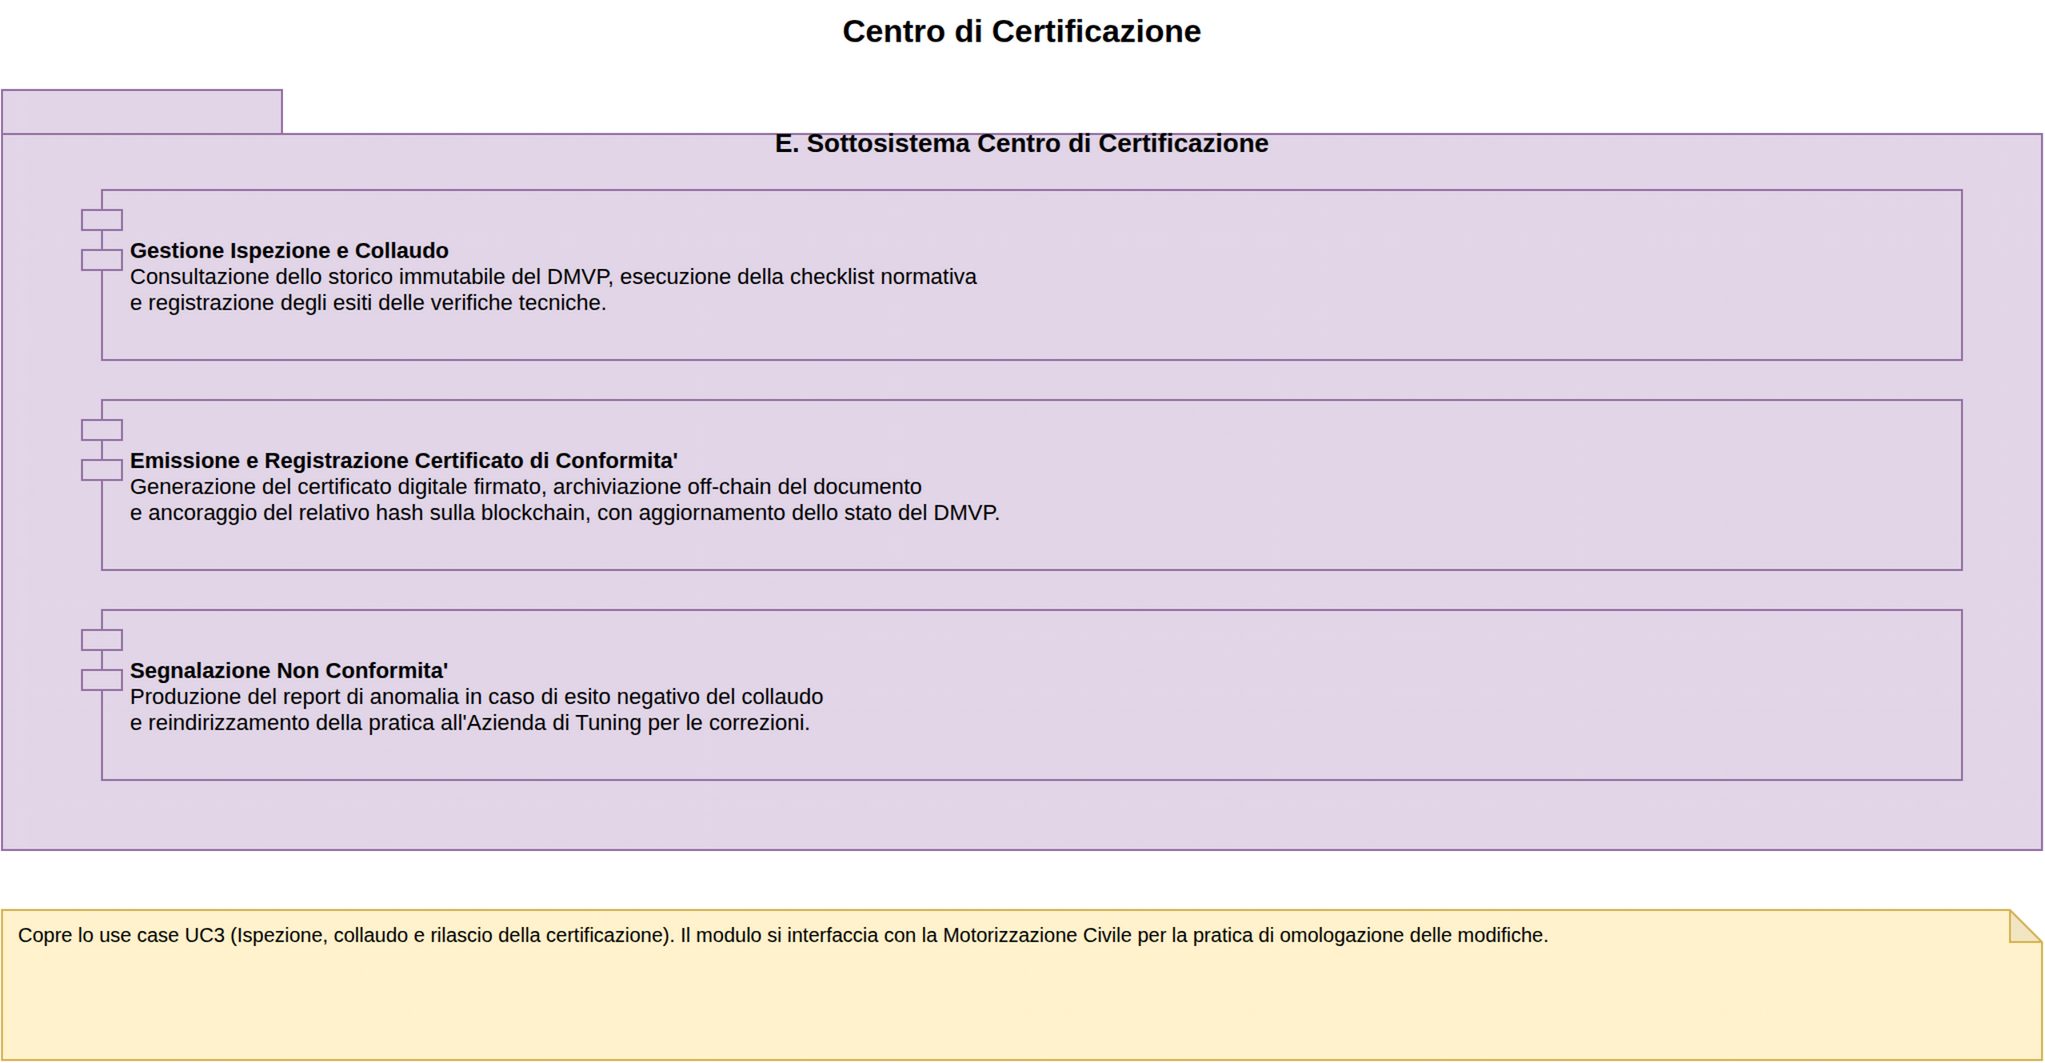
\includegraphics[width=\textwidth]{imgs/projectplan/05_sottosistema_centro_certificazione.png}
    \caption{Sottosistema Centro di Certificazione}
    \label{fig:sub-certificazione}
\end{figure}

\subsection*{Sottosistema Front-End Unificato}

Il sottosistema (Figura~\ref{fig:sub-frontend}) raccoglie l'insieme delle interfacce utente della piattaforma, realizzate come applicazione unica multi-ruolo: la separazione tra utenti B2B e B2C avviene a livello di autenticazione e di profilo autorizzativo. Esso comprende il portale web destinato a Concessionaria, Azienda di Tuning e Centro di Certificazione, l'applicazione mobile per il Cliente Privato, la console di governance dell'Intermediario e l'API Gateway, punto di ingresso unico ai micro-servizi.

\begin{figure}[H]
    \centering
    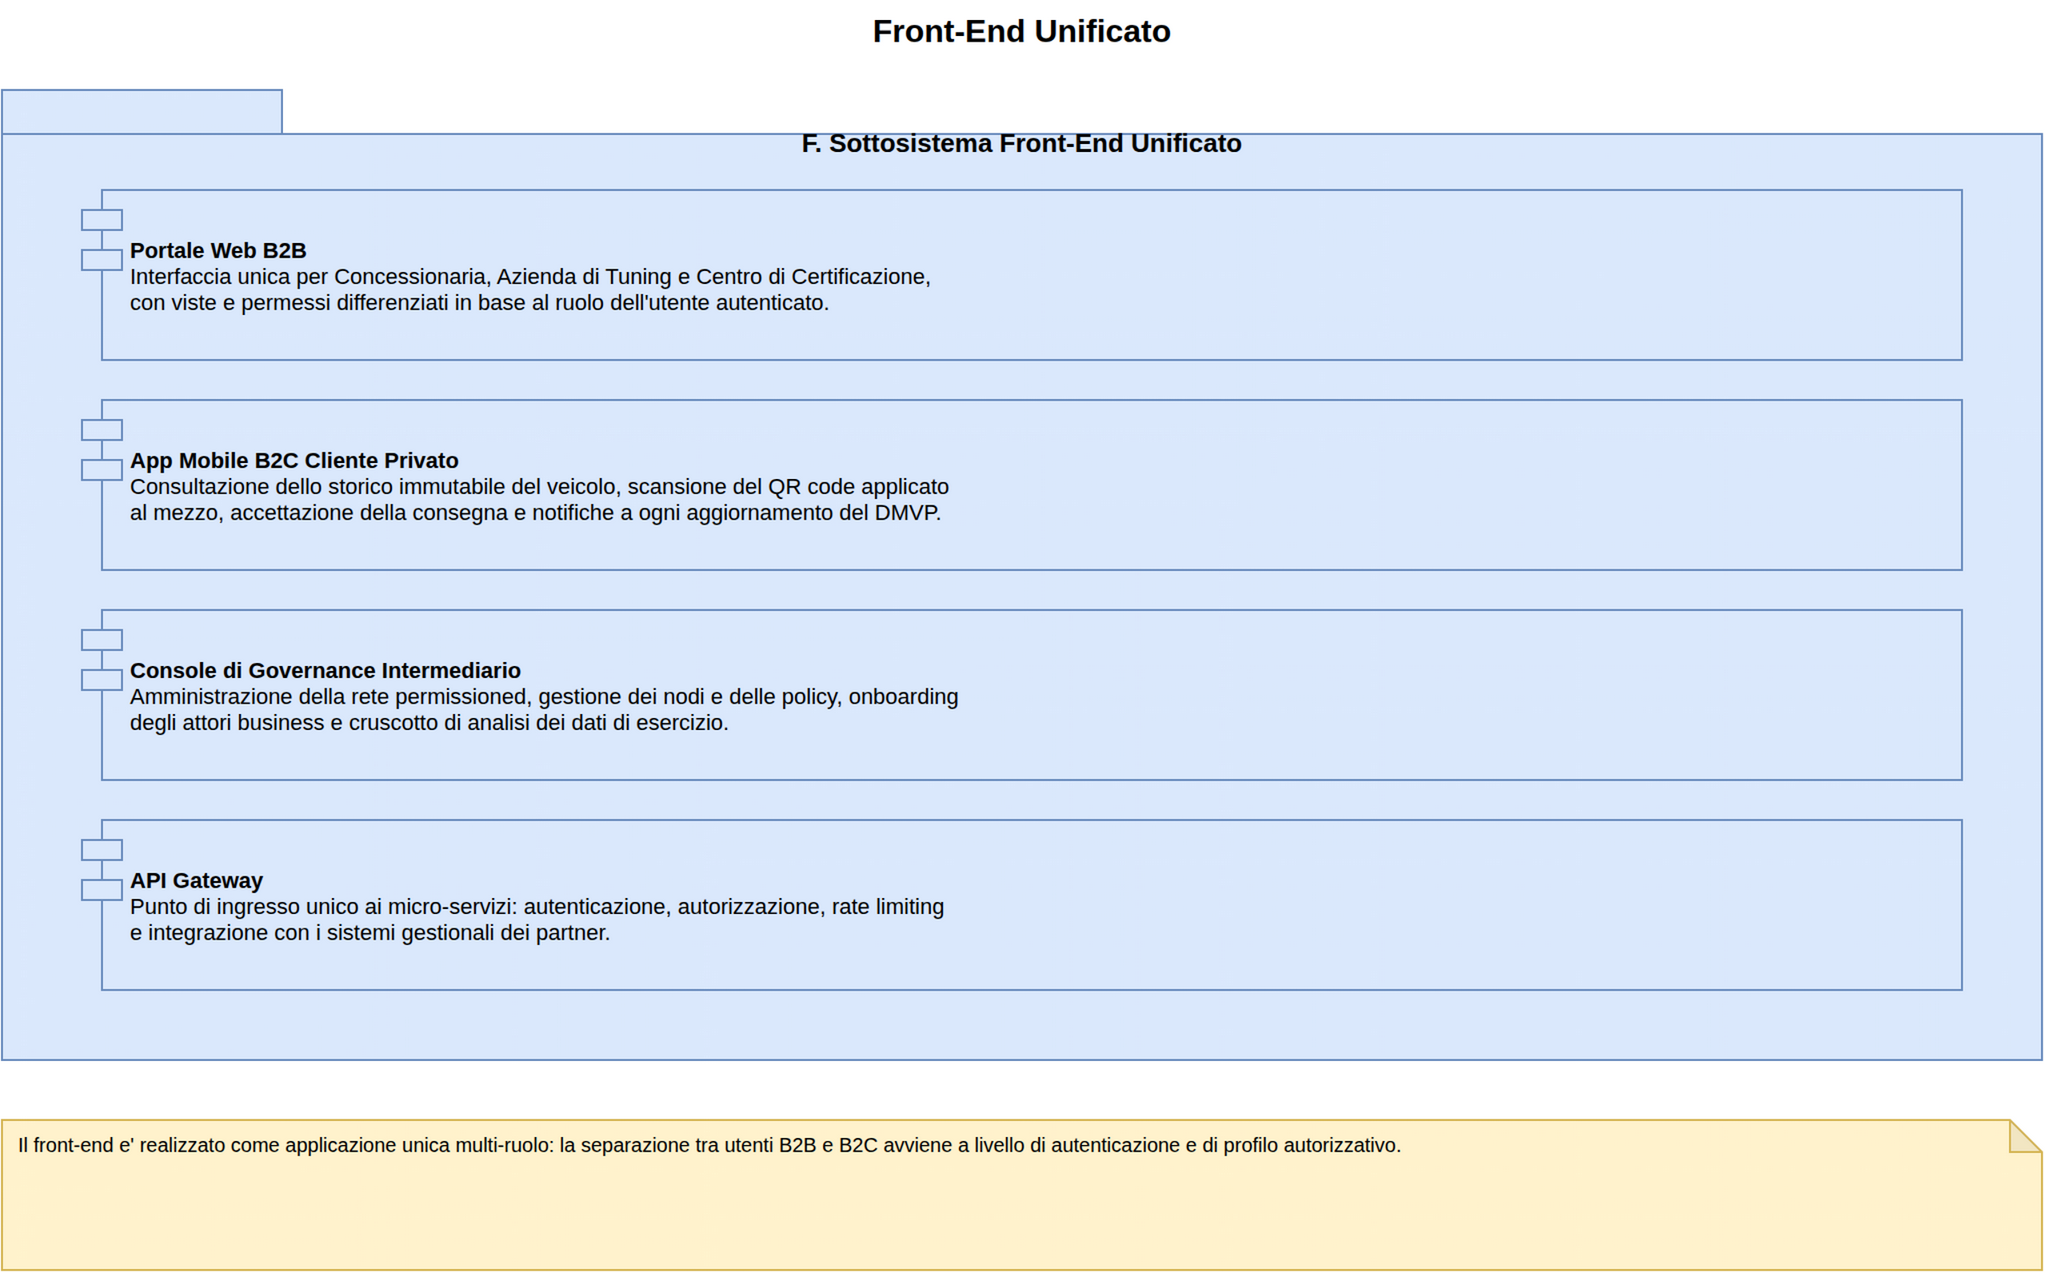
\includegraphics[width=\textwidth]{imgs/projectplan/06_sottosistema_front_end.png}
    \caption{Sottosistema Front-End Unificato}
    \label{fig:sub-frontend}
\end{figure}

\subsection*{Diagramma di Distribuzione}

Il diagramma di distribuzione riportato in Figura~\ref{fig:deployment} illustra la collocazione dei componenti sui nodi di elaborazione. Il cluster applicativo e i nodi della rete permissioned sono ospitati su infrastruttura cloud; ogni organizzazione partecipante mantiene un proprio \textit{peer} con copia del ledger, cosicché nessun attore possa alterare unilateralmente i dati registrati. I documenti e le prove multimediali restano sull'\textit{object storage} off-chain, mentre sulla catena viene scritto soltanto l'hash che ne garantisce l'integrità.

\begin{figure}[H]
    \centering
    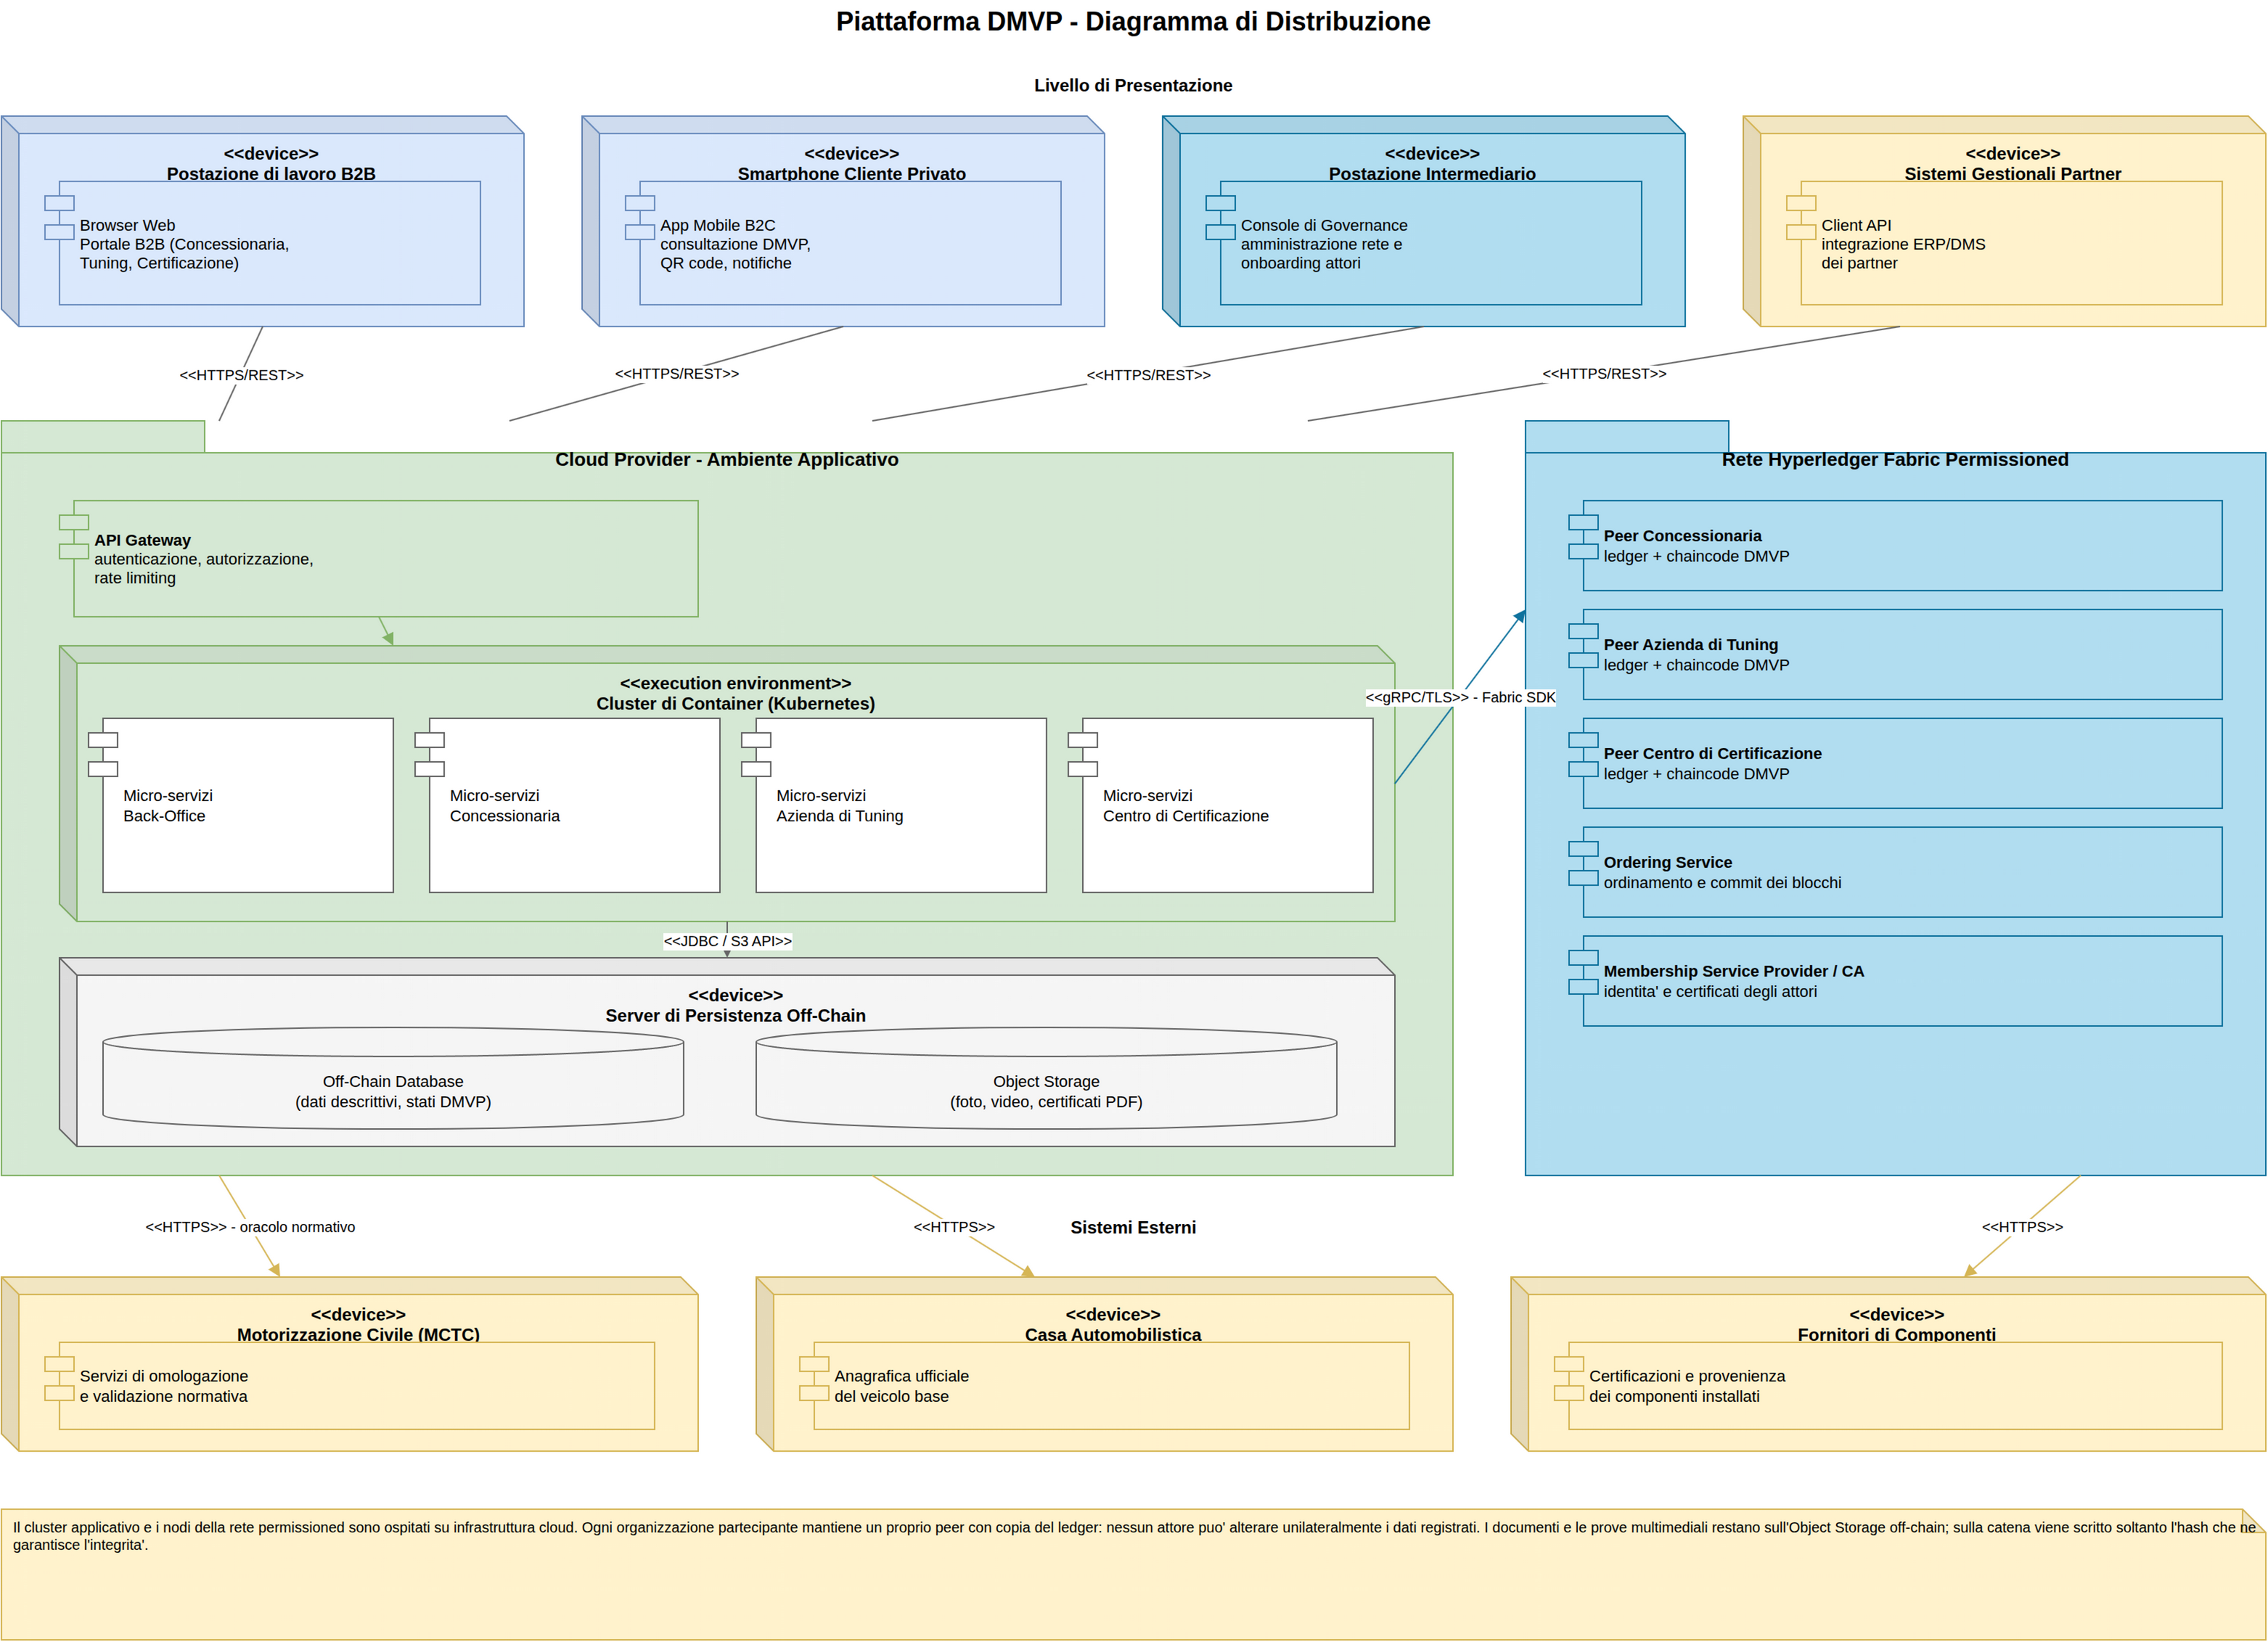
\includegraphics[width=\textwidth]{imgs/projectplan/07_deployment_diagram.png}
    \caption{Diagramma di distribuzione della piattaforma DMVP}
    \label{fig:deployment}
\end{figure}

\section{Ambienti e Tecnologie di Sviluppo}


Per lo strato di registro distribuito viene adottato \textbf{Hyperledger Fabric}, piattaforma blockchain \textit{permissioned} di riferimento per gli scenari consortili. La scelta è motivata dal modello di identità basato su \textit{Membership Service Provider} e Certification Authority, che consente all'Intermediario di verificare preventivamente gli attori ammessi alla rete, e dalle politiche di \textit{endorsement} configurabili, che permettono di stabilire quali organizzazioni debbano validare ciascuna tipologia di transazione. La logica applicativa del passaporto digitale è implementata come \textit{chaincode}, responsabile della registrazione degli hash e della gestione delle transizioni di stato del DMVP.

Per lo sviluppo dei micro-servizi di back-end viene adottato l'ambiente di runtime \textbf{Node.js} accoppiato al framework \textbf{Express}, scelto per la leggerezza, per il modello di I/O asincrono e non bloccante e per l'integrazione nativa con l'SDK di Hyperledger Fabric. Questo stack consente di gestire flussi di richieste ad alta concorrenza riducendo al minimo l'overhead computazionale del server.

Per la gestione dello strato di persistenza, l'architettura adotta un approccio ibrido che separa le informazioni strutturate dai contenuti documentali. Gli stati del DMVP, le anagrafiche degli attori e i metadati delle lavorazioni sono memorizzati in un \textbf{database off-chain}, scelto per la flessibilità dello schema e l'alta velocità di esecuzione delle query. La documentazione voluminosa (fotografie, video, schede tecniche e certificati in formato PDF) è invece delegata a un servizio di \textbf{object storage}, all'interno del quale ciascun oggetto è identificato dalla propria impronta crittografica. Sulla blockchain non vengono quindi allocati i file binari, bensì i soli hash: questa separazione ottimizza le prestazioni del database, contiene i costi di transazione e garantisce al contempo l'inalterabilità delle prove digitali raccolte.

Per il front-end si utilizza \textbf{Flutter}, framework multi-piattaforma basato sul linguaggio Dart, che consente di realizzare con un'unica base di codice sia il portale web B2B sia l'applicazione mobile destinata al Cliente Privato. Flutter si integra efficacemente con le architetture API REST e adotta il pattern MVVM (\textit{Model-View-ViewModel}), in cui il ViewModel gestisce lo stato reattivo dei componenti dell'interfaccia.

L'intero ambiente applicativo è containerizzato mediante \textbf{Docker} e orchestrato tramite \textbf{Kubernetes}, soluzione che garantisce la scalabilità orizzontale dei singoli micro-servizi e l'isolamento dei sottosistemi.

Per lo sviluppo della soluzione vengono infine impiegati i seguenti strumenti:

\begin{itemize}
    \item \textbf{Visual Studio Code}: adottato come ambiente di sviluppo integrato unificato, sia per la componente back-end sia per il front-end in Flutter. La scelta è strategica in quanto garantisce un ambiente leggero, flessibile e altamente personalizzabile, senza rinunciare a strumenti avanzati di refactoring e di completamento intelligente del codice.
    \item \textbf{GitHub}: impiegato come piattaforma di hosting e sistema di controllo di versione distribuito. Semplifica la gestione, il \textit{branching} e la tracciabilità delle modifiche apportate al codice sorgente, consentendo una collaborazione efficiente e parallela tra i membri del team e permettendo di automatizzare le \textit{code review} tramite \textit{Pull Request}.
\end{itemize}

\section{Pianificazione della Prima Fase del Progetto: Sviluppo della Piattaforma}

Lo sviluppo della piattaforma è suddiviso in sette Task principali, ciascuno articolato in diversi sub-task funzionali. Questa scomposizione consente una gestione modulare delle attività e una chiara attribuzione delle responsabilità in base alle competenze del team. La suddivisione dei Task e dei relativi sub-task è dettagliata nella Tabella~\ref{tab:task-fase1}.

\begin{table}[H]
\centering
\small
\makebox[\textwidth][c]{%
\begin{tabular}{clllrr}
\hline
\textbf{Cod.} & \textbf{Task / Sub-task} & \textbf{Gruppo} & \textbf{Periodo} & \textbf{O/P} & \textbf{A/P} \\
\hline
\textbf{A} & \textbf{Organizzazione del Progetto} & Gruppo 0 & & \textbf{3.066} & \textbf{1,75} \\
A1 & Set-Up del Progetto & & sett.\ 1--2 & 438 & 0,25 \\
A2 & Gruppi e Ambienti di Sviluppo & & sett.\ 3--8 & 2.628 & 1,50 \\
\hline
\textbf{B} & \textbf{Sottosistema Back-Office} & Gruppo 1 & & \textbf{5.636} & \textbf{3,22} \\
B1 & Identity \& Access Management e Onboarding & & sett.\ 9--12 & 730 & 0,42 \\
B2 & DMVP Registry e Ciclo di Vita del Passaporto & & sett.\ 13--20 & 1.402 & 0,80 \\
B3 & Off-Chain Store Manager e Blockchain Gateway & & sett.\ 21--30 & 1.752 & 1,00 \\
B4 & Ricerca/Verifica, Notifiche e Integrazione & & sett.\ 31--40 & 1.752 & 1,00 \\
\hline
\textbf{C} & \textbf{Sottosistema Concessionaria} & Gruppo 2 & & \textbf{3.139} & \textbf{1,79} \\
C1 & Gestione Dati Veicolo Base & & sett.\ 9--12 & 511 & 0,29 \\
C2 & Inizializzazione DMVP e Richiesta di Tuning & & sett.\ 13--24 & 1.577 & 0,90 \\
C3 & Gestione Consegna e Trasferimento DMVP & & sett.\ 25--32 & 1.051 & 0,60 \\
\hline
\textbf{D} & \textbf{Sottosistema Azienda di Tuning} & Gruppo 2 & & \textbf{1.051} & \textbf{0,60} \\
D1 & Registrazione Modifiche e Seriali Componenti & & sett.\ 33--36 & 526 & 0,30 \\
D2 & Acquisizione Prove Multimediali e Documentazione & & sett.\ 37--40 & 526 & 0,30 \\
\hline
\textbf{E} & \textbf{Sottosistema Centro di Certificazione} & Gruppo 3 & & \textbf{1.051} & \textbf{0,60} \\
E1 & Gestione Ispezione e Collaudo & & sett.\ 33--36 & 526 & 0,30 \\
E2 & Emissione e Registrazione del Certificato & & sett.\ 37--40 & 526 & 0,30 \\
\hline
\textbf{F} & \textbf{Sottosistema Front-End Unificato} & Gruppo 3 & & \textbf{3.139} & \textbf{1,79} \\
F1 & Portale Web B2B & & sett.\ 9--18 & 1.299 & 0,74 \\
F2 & App Mobile B2C Cliente Privato & & sett.\ 19--26 & 1.051 & 0,60 \\
F3 & Console di Governance Intermediario e Analytics & & sett.\ 27--32 & 788 & 0,45 \\
\hline
\textbf{G} & \textbf{Integrazione/Testing complessivo e Deployment} & Gruppo 0 & & \textbf{3.504} & \textbf{2,00} \\
G1 & Integrazione/Testing complessivo & & sett.\ 41--46 & 2.628 & 1,50 \\
G2 & Deployment & & sett.\ 47--48 & 876 & 0,50 \\
\hline
& \textbf{TOTALE FASE 1} & & & \textbf{20.586} & \textbf{11,75} \\
\hline
\end{tabular}}
\caption{Task e sub-task della Prima Fase}
\label{tab:task-fase1}
\end{table}

Nella pianificazione del progetto si fa riferimento alla metodologia \textbf{Agile}, e in particolare a \textbf{Scrum}, framework di processo iterativo e incrementale ampiamente consolidato nell'ingegneria del software.

Scrum prevede di suddividere il ciclo di vita dello sviluppo in periodi di lavoro brevi e ben definiti, noti come \textbf{Sprint}, al termine dei quali viene rilasciato un incremento di software funzionante, testato e potenzialmente rilasciabile. Questo approccio consente di definire in dettaglio le attività a breve termine e include una serie di cerimonie progettate per monitorare costantemente l'avanzamento del lavoro, minimizzare i rischi operativi e favorire momenti di revisione e miglioramento continuo. Nel presente progetto la durata di uno Sprint è fissata in \textbf{due settimane}, pari a 73 O/P per risorsa a tempo pieno.

Un Team Scrum è composto da tre figure chiave:

\begin{itemize}
    \item \textbf{Product Owner}: rappresenta la voce degli stakeholder e dei clienti finali, assicurandosi che il team sviluppi soluzioni orientate al valore di business e ordinando il \textit{Product Backlog} in base alle priorità strategiche. Nel presente progetto tale ruolo è assunto dal Project Manager.
    \item \textbf{Development Team}: il gruppo cross-funzionale di professionisti che si occupa materialmente della progettazione, dell'implementazione e del testing del software.
    \item \textbf{Scrum Master}: agisce come leader al servizio del team, con il compito di diffondere la cultura Agile, ottimizzare i processi interni e rimuovere tempestivamente gli impedimenti che potrebbero rallentare il raggiungimento degli obiettivi di Sprint. Tale ruolo è assunto dal Software Architect.
\end{itemize}

Ogni Sprint inizia con una riunione di \textit{Sprint Planning}, durante la quale vengono determinati gli obiettivi del ciclo e stimate le risorse necessarie per completarli, estraendole dal backlog. Al termine di ogni Sprint, durante la \textit{Sprint Review}, il team consegna e dimostra una versione operativa del prodotto, procedendo poi alla \textit{Sprint Retrospective} per analizzare e ottimizzare i processi di lavoro interni.

Per quanto concerne la pianificazione delle risorse umane impiegate nella prima fase, si considera l'impiego delle seguenti figure professionali:

\begin{itemize}
    \item \textbf{Un Project Manager (PM)}, coinvolto in tutte le macro-attività del ciclo di vita con il ruolo metodologico di Product Owner, per garantire la corrispondenza dei moduli sviluppati alle specifiche di business individuate nella modellazione.
    \item \textbf{Un Software Architect (SA)}, presente trasversalmente in tutti i task operativi con il ruolo di Scrum Master, per supervisionare la coerenza tecnica dell'architettura a micro-servizi e della componente blockchain e per guidare l'intero team di sviluppo.
    \item \textbf{Quattro Full Stack Developer (FSD)}, distribuiti all'interno dei gruppi di lavoro e responsabili primari dell'implementazione delle logiche computazionali del Back-Office, della scrittura del chaincode e dell'integrazione con la rete permissioned.
    \item \textbf{Sei Full Stack Developer Junior (FSDJ)}, distribuiti nei vari team e focalizzati sulla realizzazione dei moduli applicativi di supporto e delle interfacce in Flutter, lavorando in sinergia con il back-end.
\end{itemize}

I gruppi di lavoro individuati sono quattro e vengono riassunti in Figura~\ref{fig:gruppi-fase1} e nella Tabella~\ref{tab:gruppi-fase1}.

\begin{figure}[H]
    \centering
    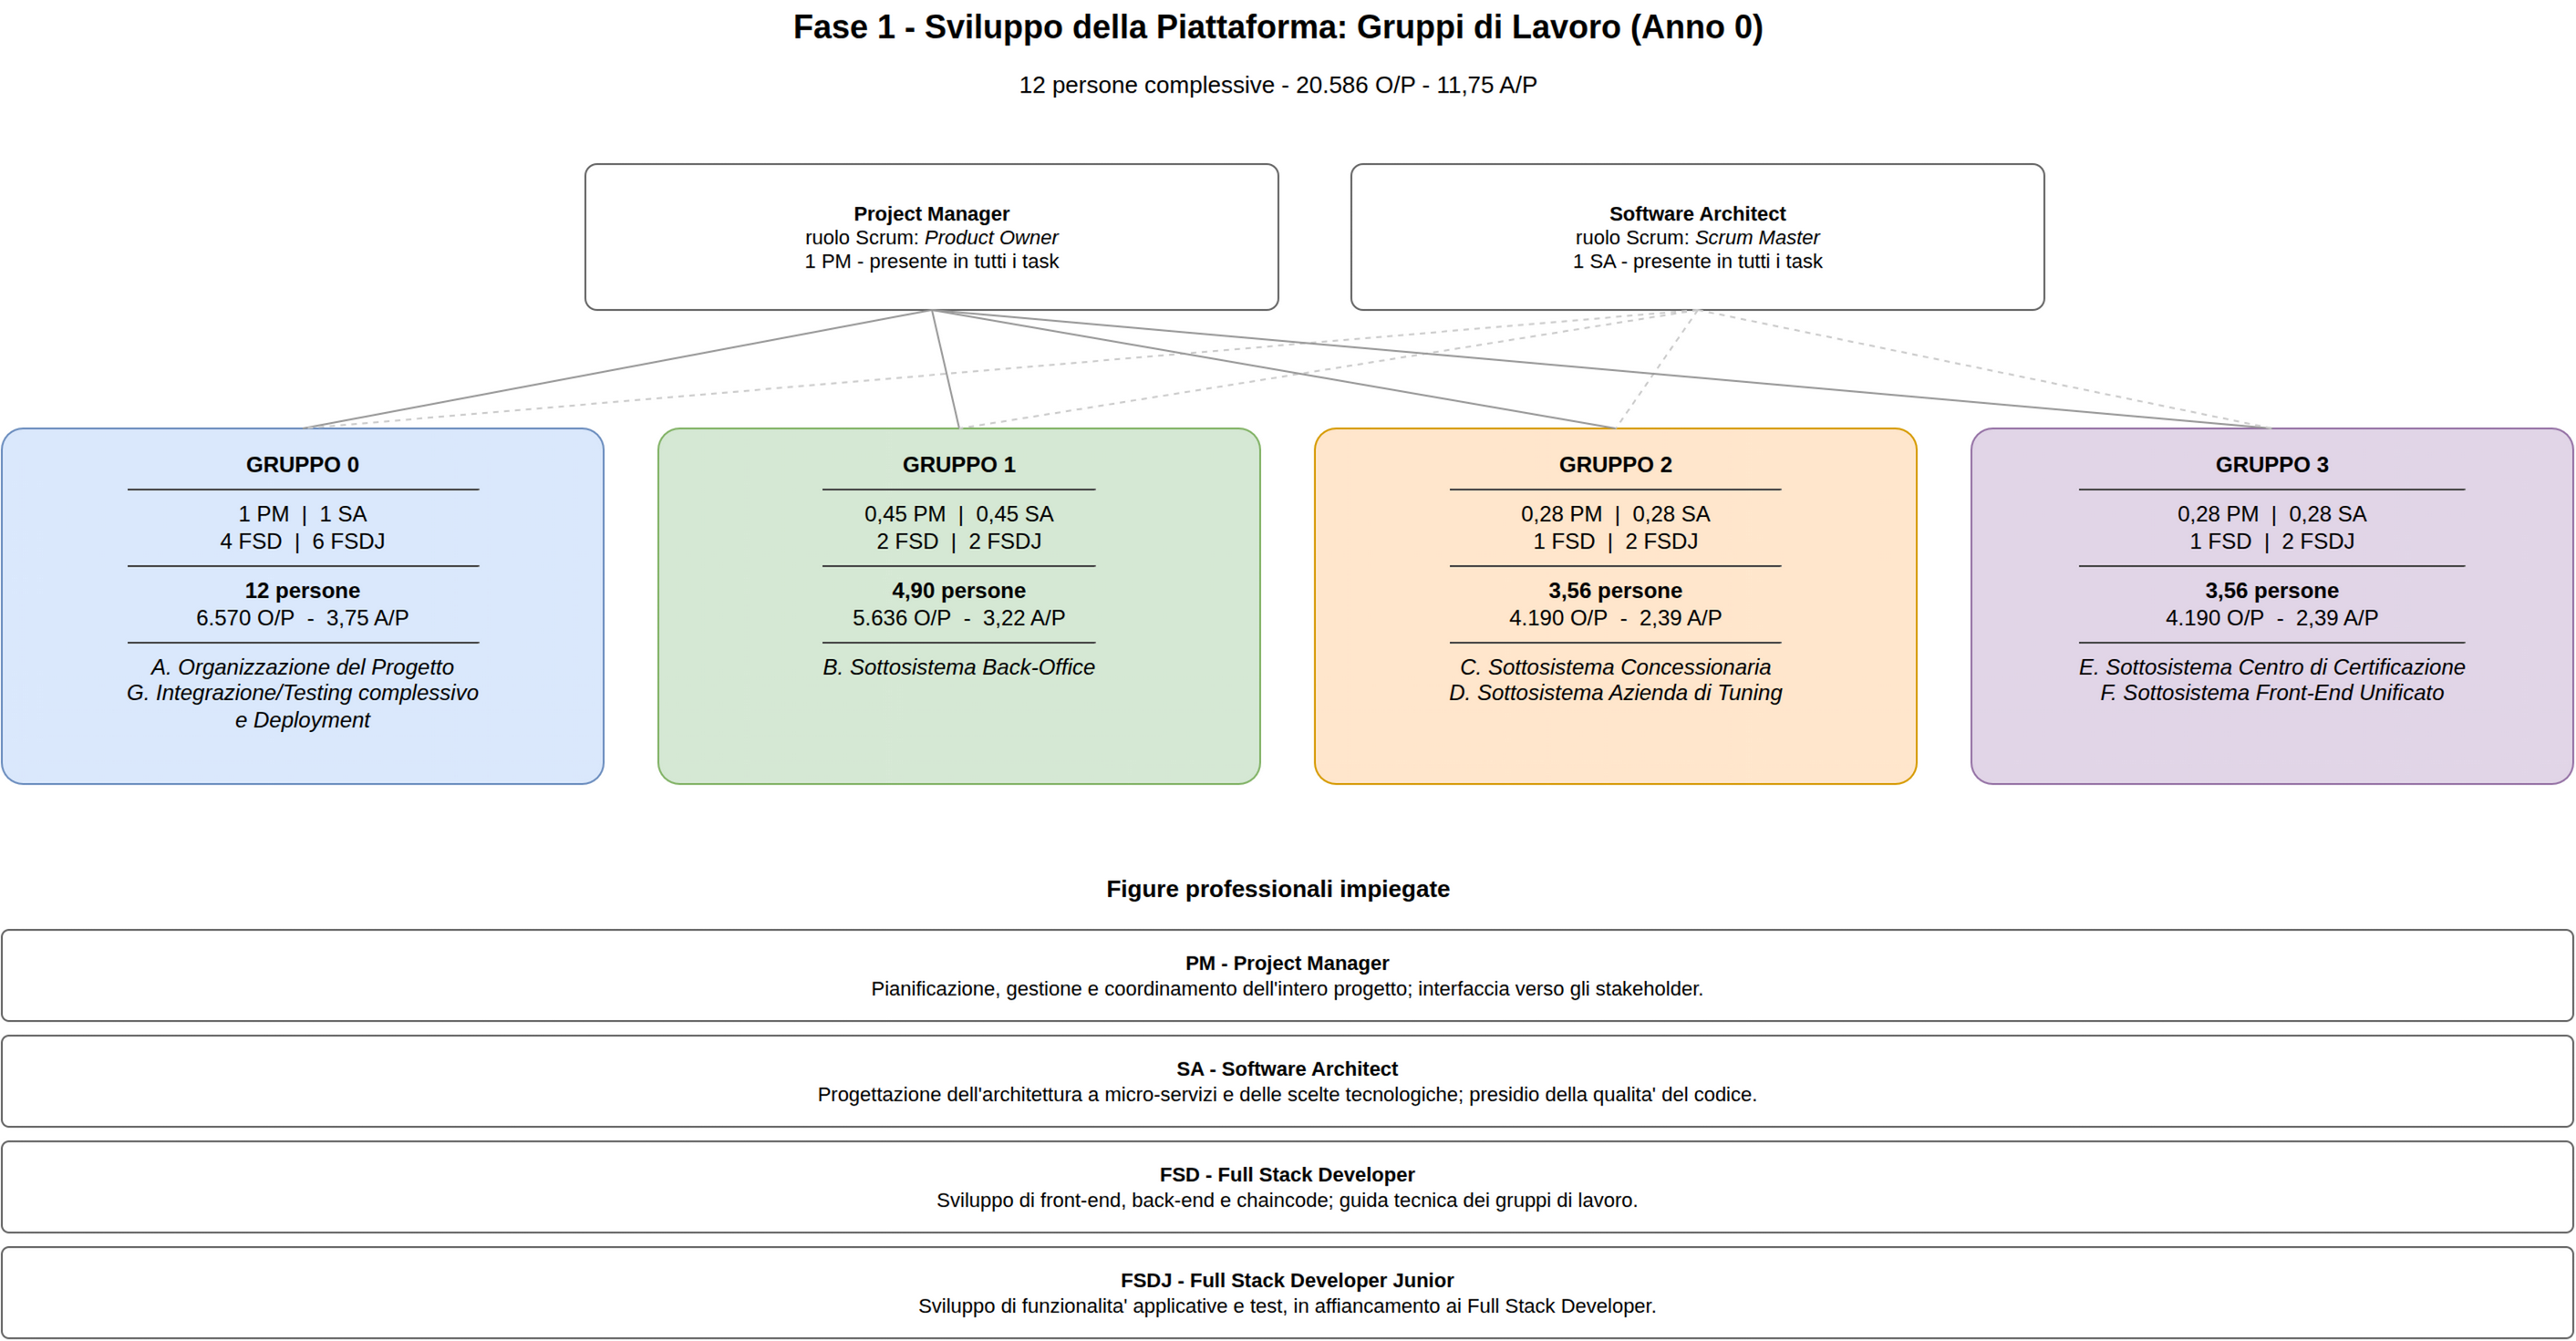
\includegraphics[width=\textwidth]{imgs/projectplan/08_gruppi_fase1.png}
    \caption{Gruppi di lavoro della Fase 1}
    \label{fig:gruppi-fase1}
\end{figure}

\begin{table}[H]
\centering
\small
\makebox[\textwidth][c]{%
\begin{tabular}{llll rr}
\hline
\textbf{Gruppo} & \textbf{Persone} & \textbf{Tipologia} & \textbf{Task} & \textbf{O/P} & \textbf{A/P} \\
\hline
Gruppo 0 & 12,00 & 1 PM, 1 SA, 4 FSD, 6 FSDJ & A, G & 6.570 & 3,75 \\
Gruppo 1 & 4,90 & 0,45 PM, 0,45 SA, 2 FSD, 2 FSDJ & B & 5.636 & 3,22 \\
Gruppo 2 & 3,56 & 0,28 PM, 0,28 SA, 1 FSD, 2 FSDJ & C, D & 4.190 & 2,39 \\
Gruppo 3 & 3,56 & 0,28 PM, 0,28 SA, 1 FSD, 2 FSDJ & E, F & 4.190 & 2,39 \\
\hline
\textbf{TOTALE} & \textbf{12} & 1 PM, 1 SA, 4 FSD, 6 FSDJ & A--G & \textbf{20.586} & \textbf{11,75} \\
\hline
\end{tabular}}
\caption{Composizione e impegno dei gruppi di lavoro della Fase 1}
\label{tab:gruppi-fase1}
\end{table}

I Gruppi 1, 2 e 3 lavorano in parallelo sui rispettivi sottosistemi, mentre il Gruppo 0 coincide con l'intero organico ed è impegnato nelle attività iniziali di organizzazione e nelle attività finali di integrazione, testing e deployment. Il Project Manager e il Software Architect sono ripartiti tra i gruppi in quota proporzionale all'impegno richiesto da ciascun sottosistema.

Il diagramma di GANTT della prima fase, articolato sulle 48 settimane dell'Anno 0 --- raggruppate nei dodici mesi di calendario e scandite in Sprint di due settimane ciascuno --- è riportato in Figura~\ref{fig:gantt-fase1}.

\begin{figure}[H]
    \centering
    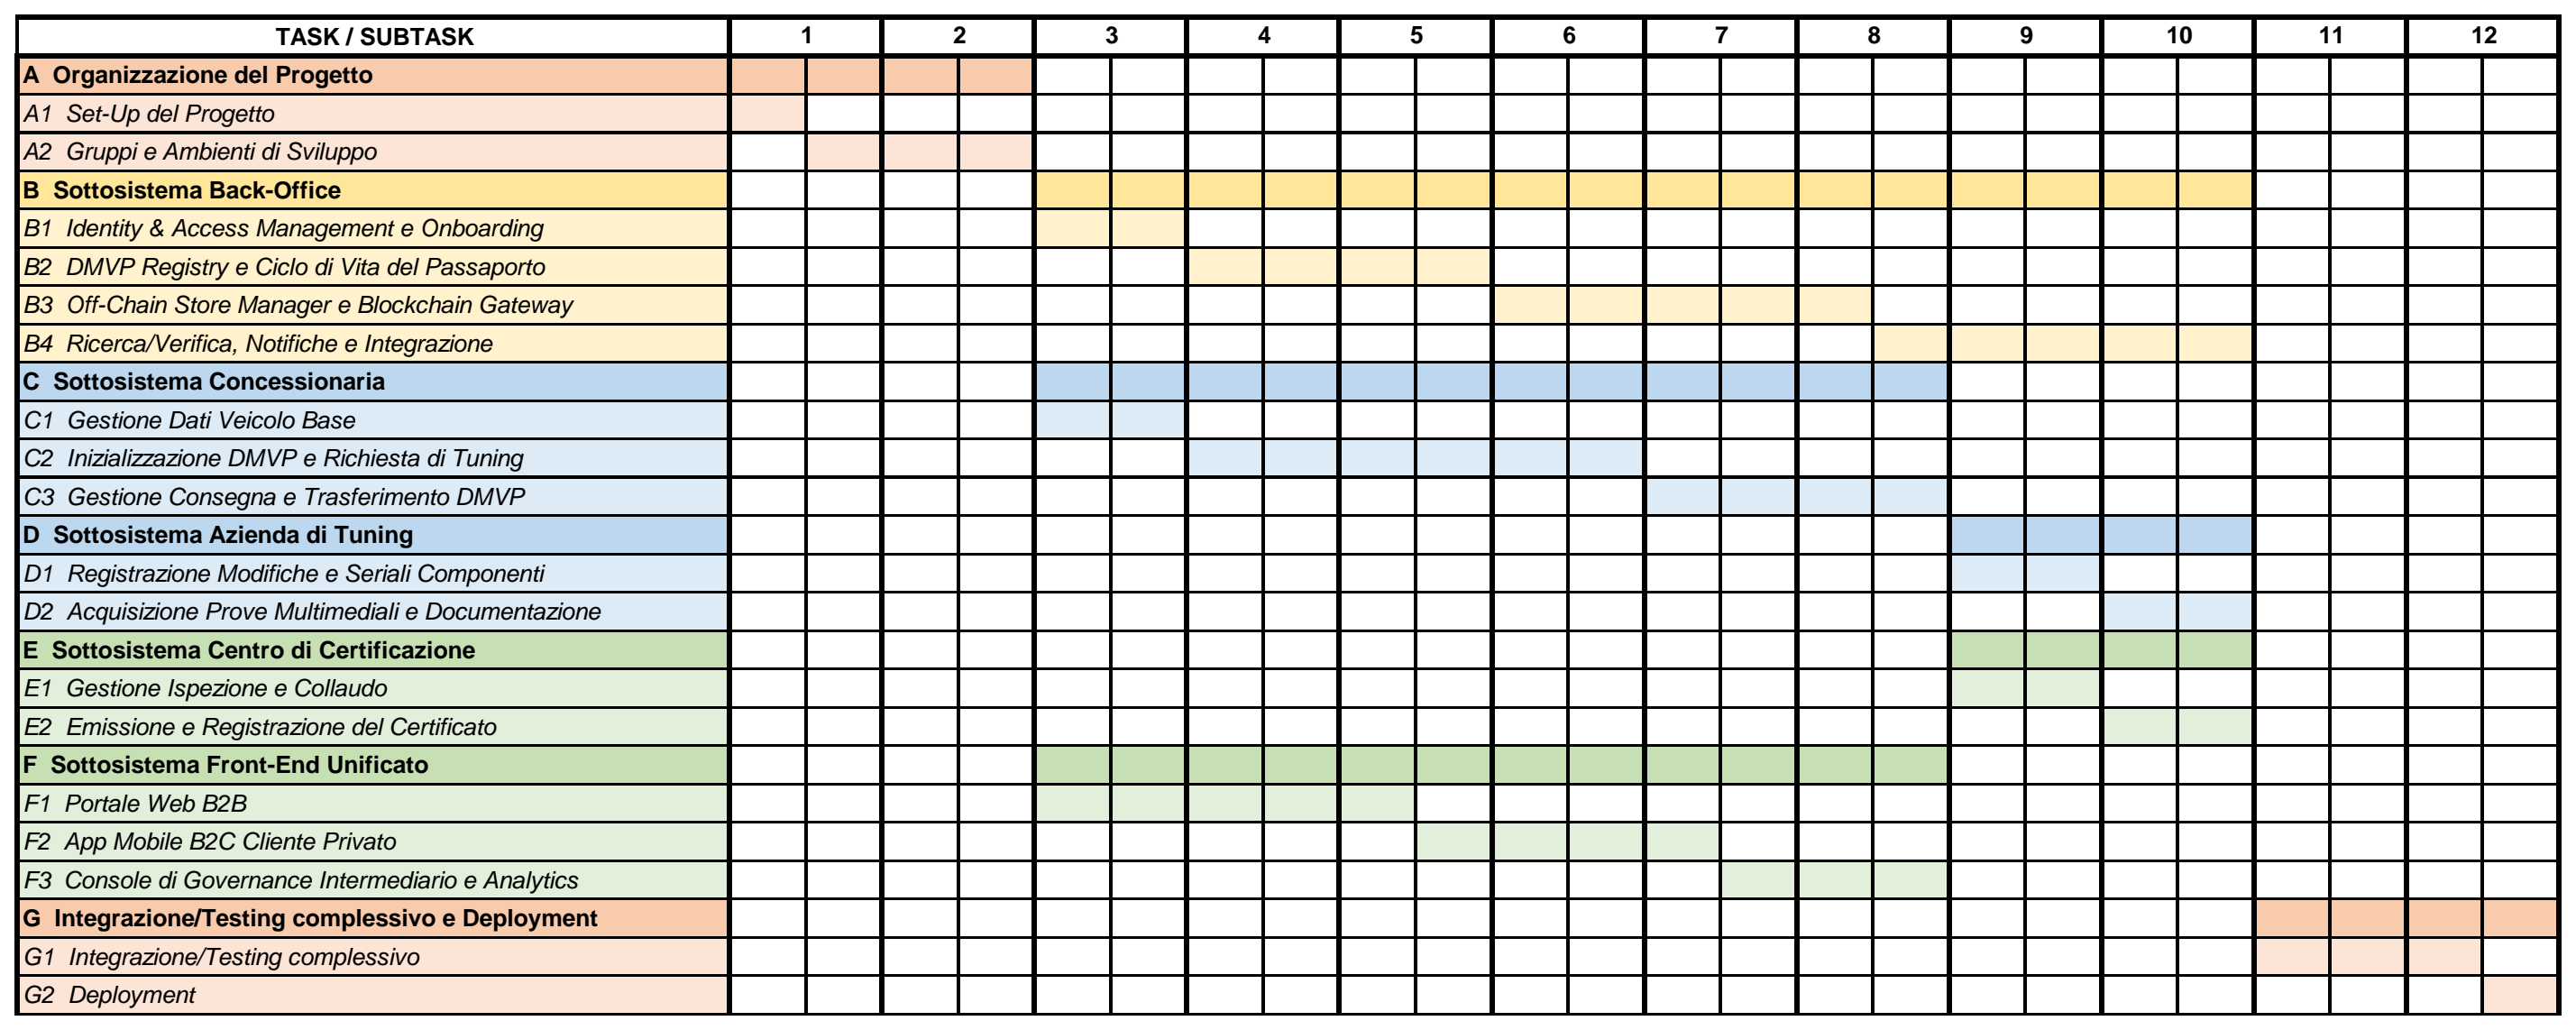
\includegraphics[width=\textwidth]{imgs/gantt/gantt_fase1/gantt_fase1.png}
    \caption{Diagramma di GANTT della Fase 1}
    \label{fig:gantt-fase1}
\end{figure}

Le diverse tipologie di risorsa vengono impegnate all'interno dei vari task come mostrato nelle Figure~\ref{fig:impegno-pm-fase1}, \ref{fig:impegno-sa-fase1}, \ref{fig:impegno-fsd-fase1}, \ref{fig:impegno-fsdj-fase1} e~\ref{fig:impegno-totale-fase1}. Si osservi che nelle prime due settimane, dedicate al solo Set-Up del Progetto, risultano operativi il Project Manager, il Software Architect e i quattro Full Stack Developer, mentre i sei Full Stack Developer Junior vengono inseriti a partire dalla terza settimana, contestualmente alla costituzione dei gruppi e alla predisposizione degli ambienti di sviluppo.

\begin{figure}[H]
    \centering
    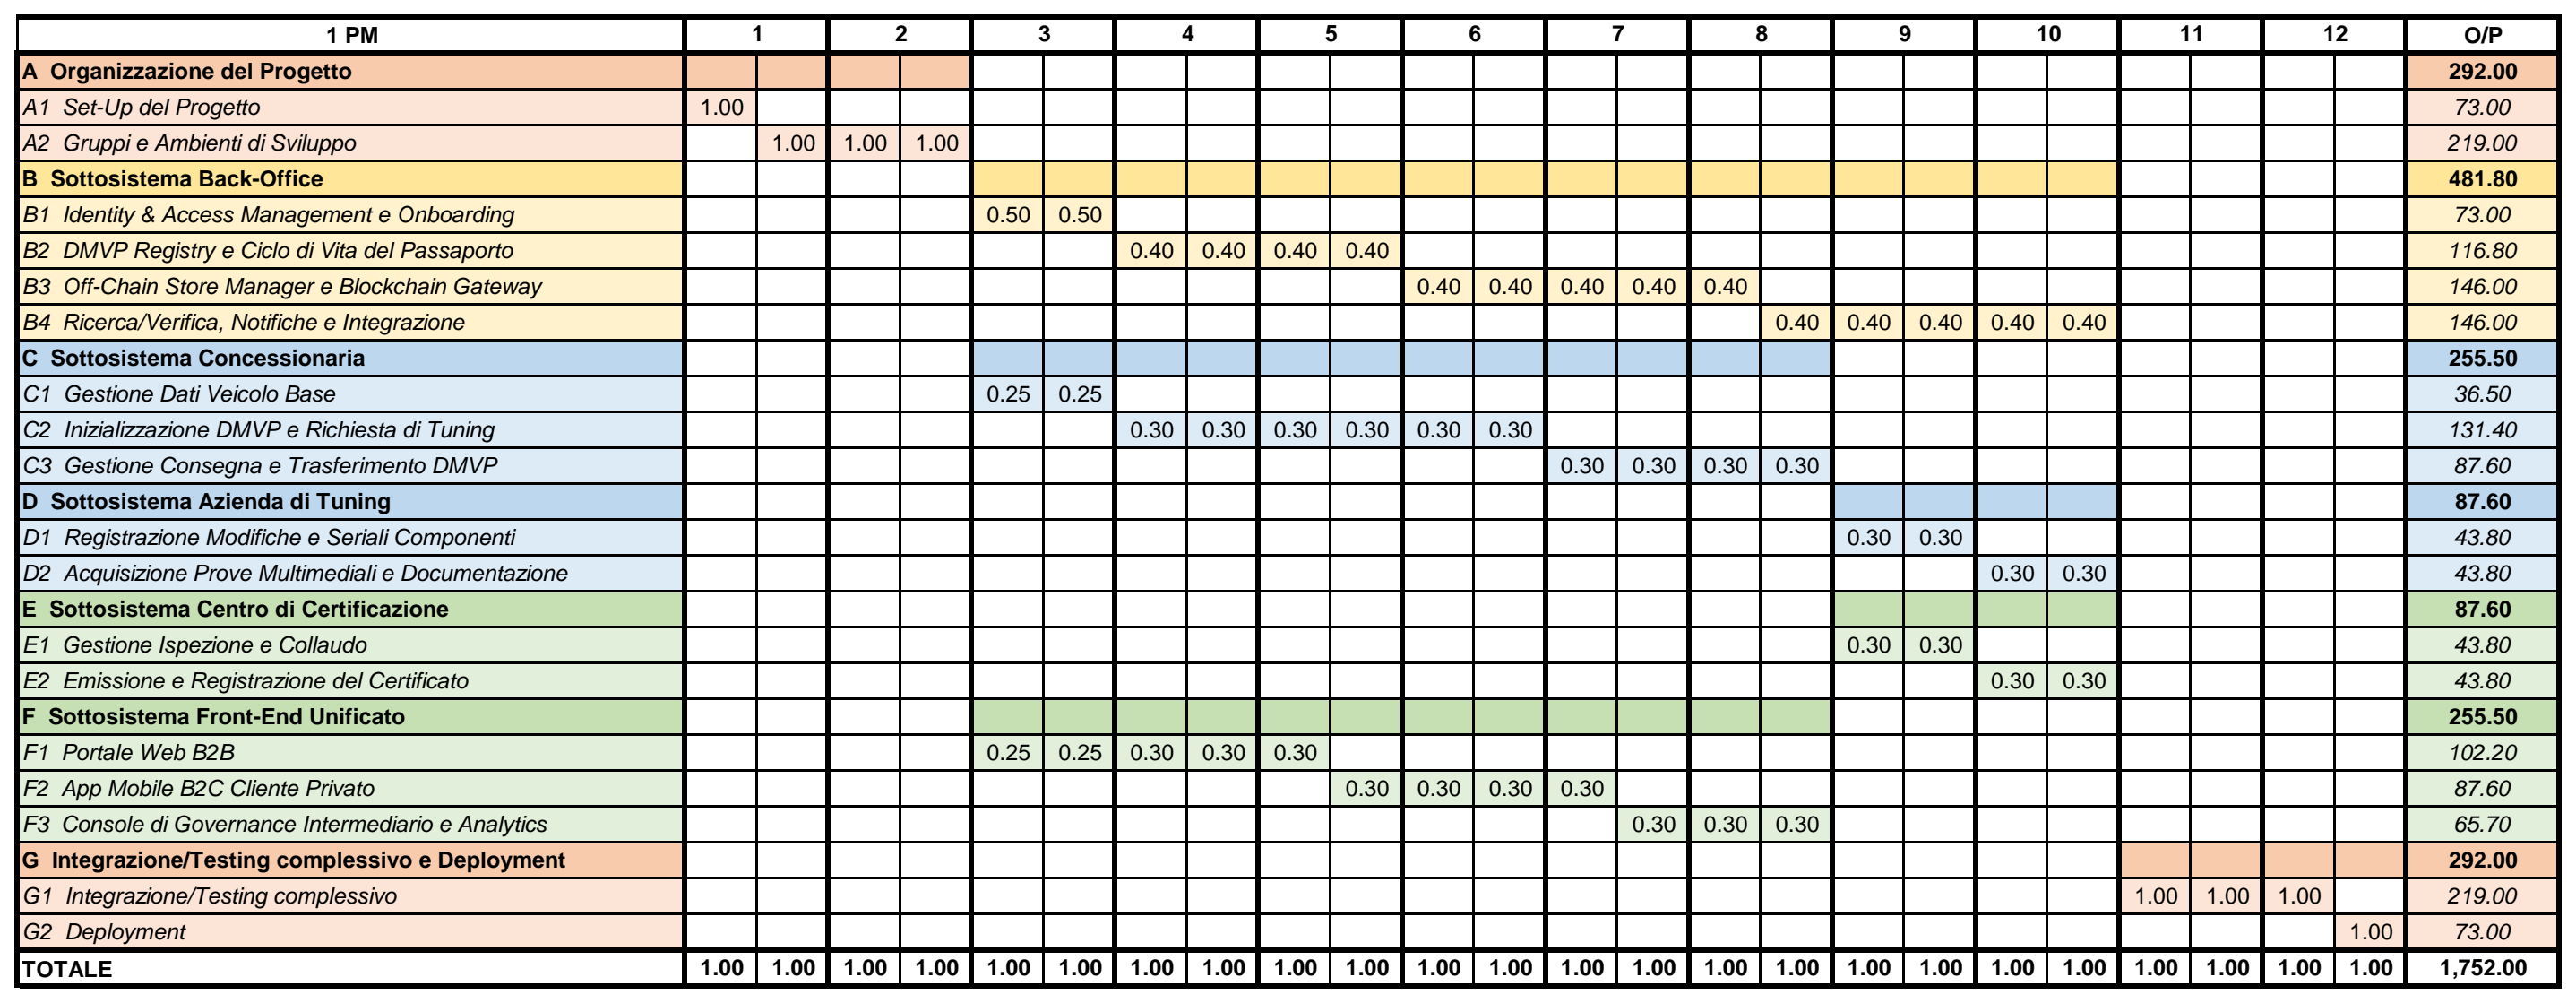
\includegraphics[width=\textwidth]{imgs/gantt/gantt_fase1/gantt_fase1_PM.png}
    \caption{Impegno del Project Manager nella Fase 1}
    \label{fig:impegno-pm-fase1}
\end{figure}
\begin{figure}[H]
    \centering
    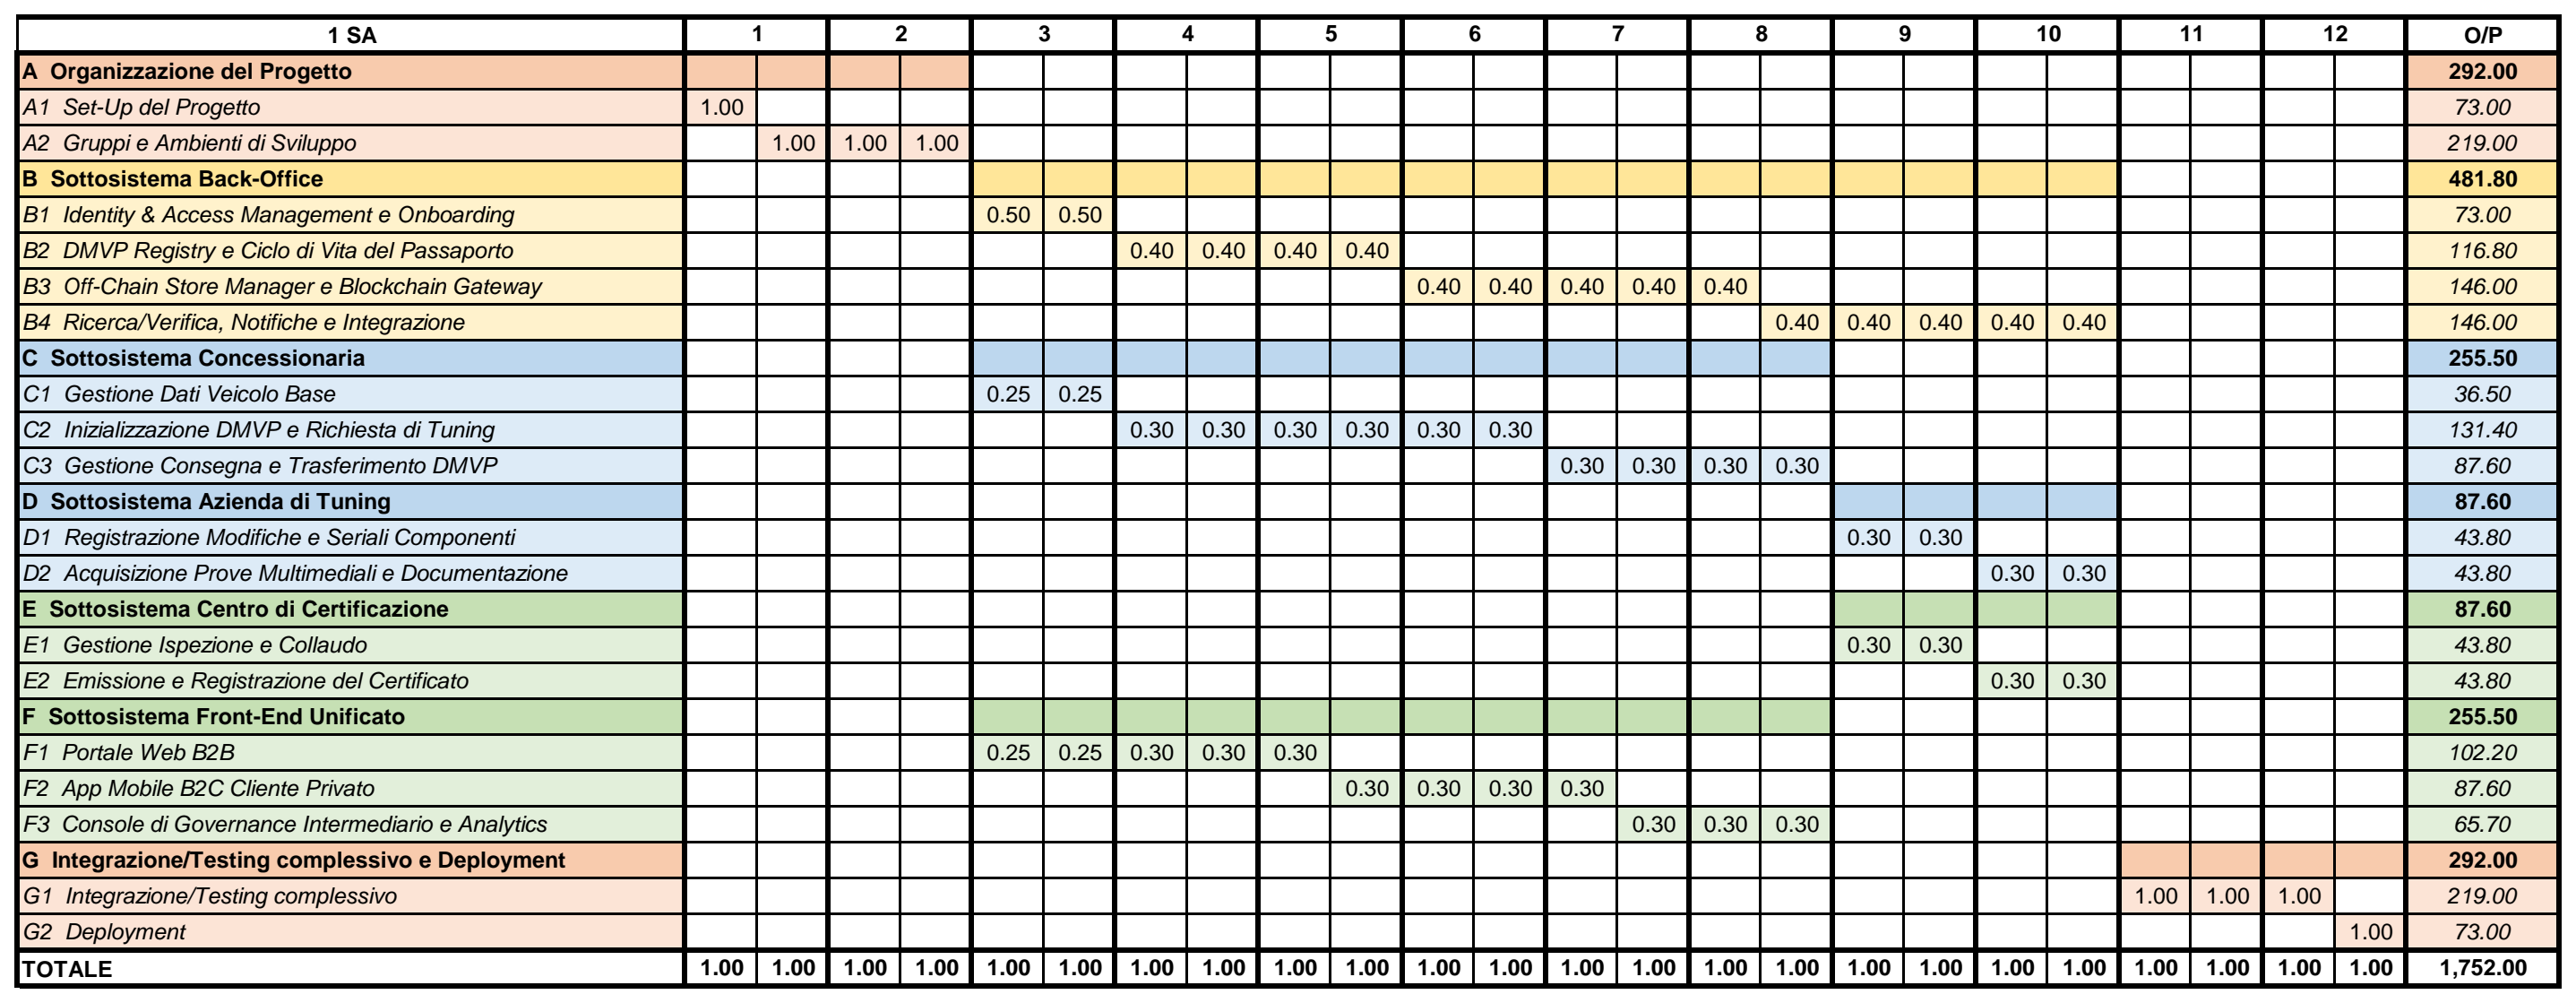
\includegraphics[width=\textwidth]{imgs/gantt/gantt_fase1/gantt_fase1_SA.png}
    \caption{Impegno del Software Architect nella Fase 1}
    \label{fig:impegno-sa-fase1}
\end{figure}
\begin{figure}[H]
    \centering
    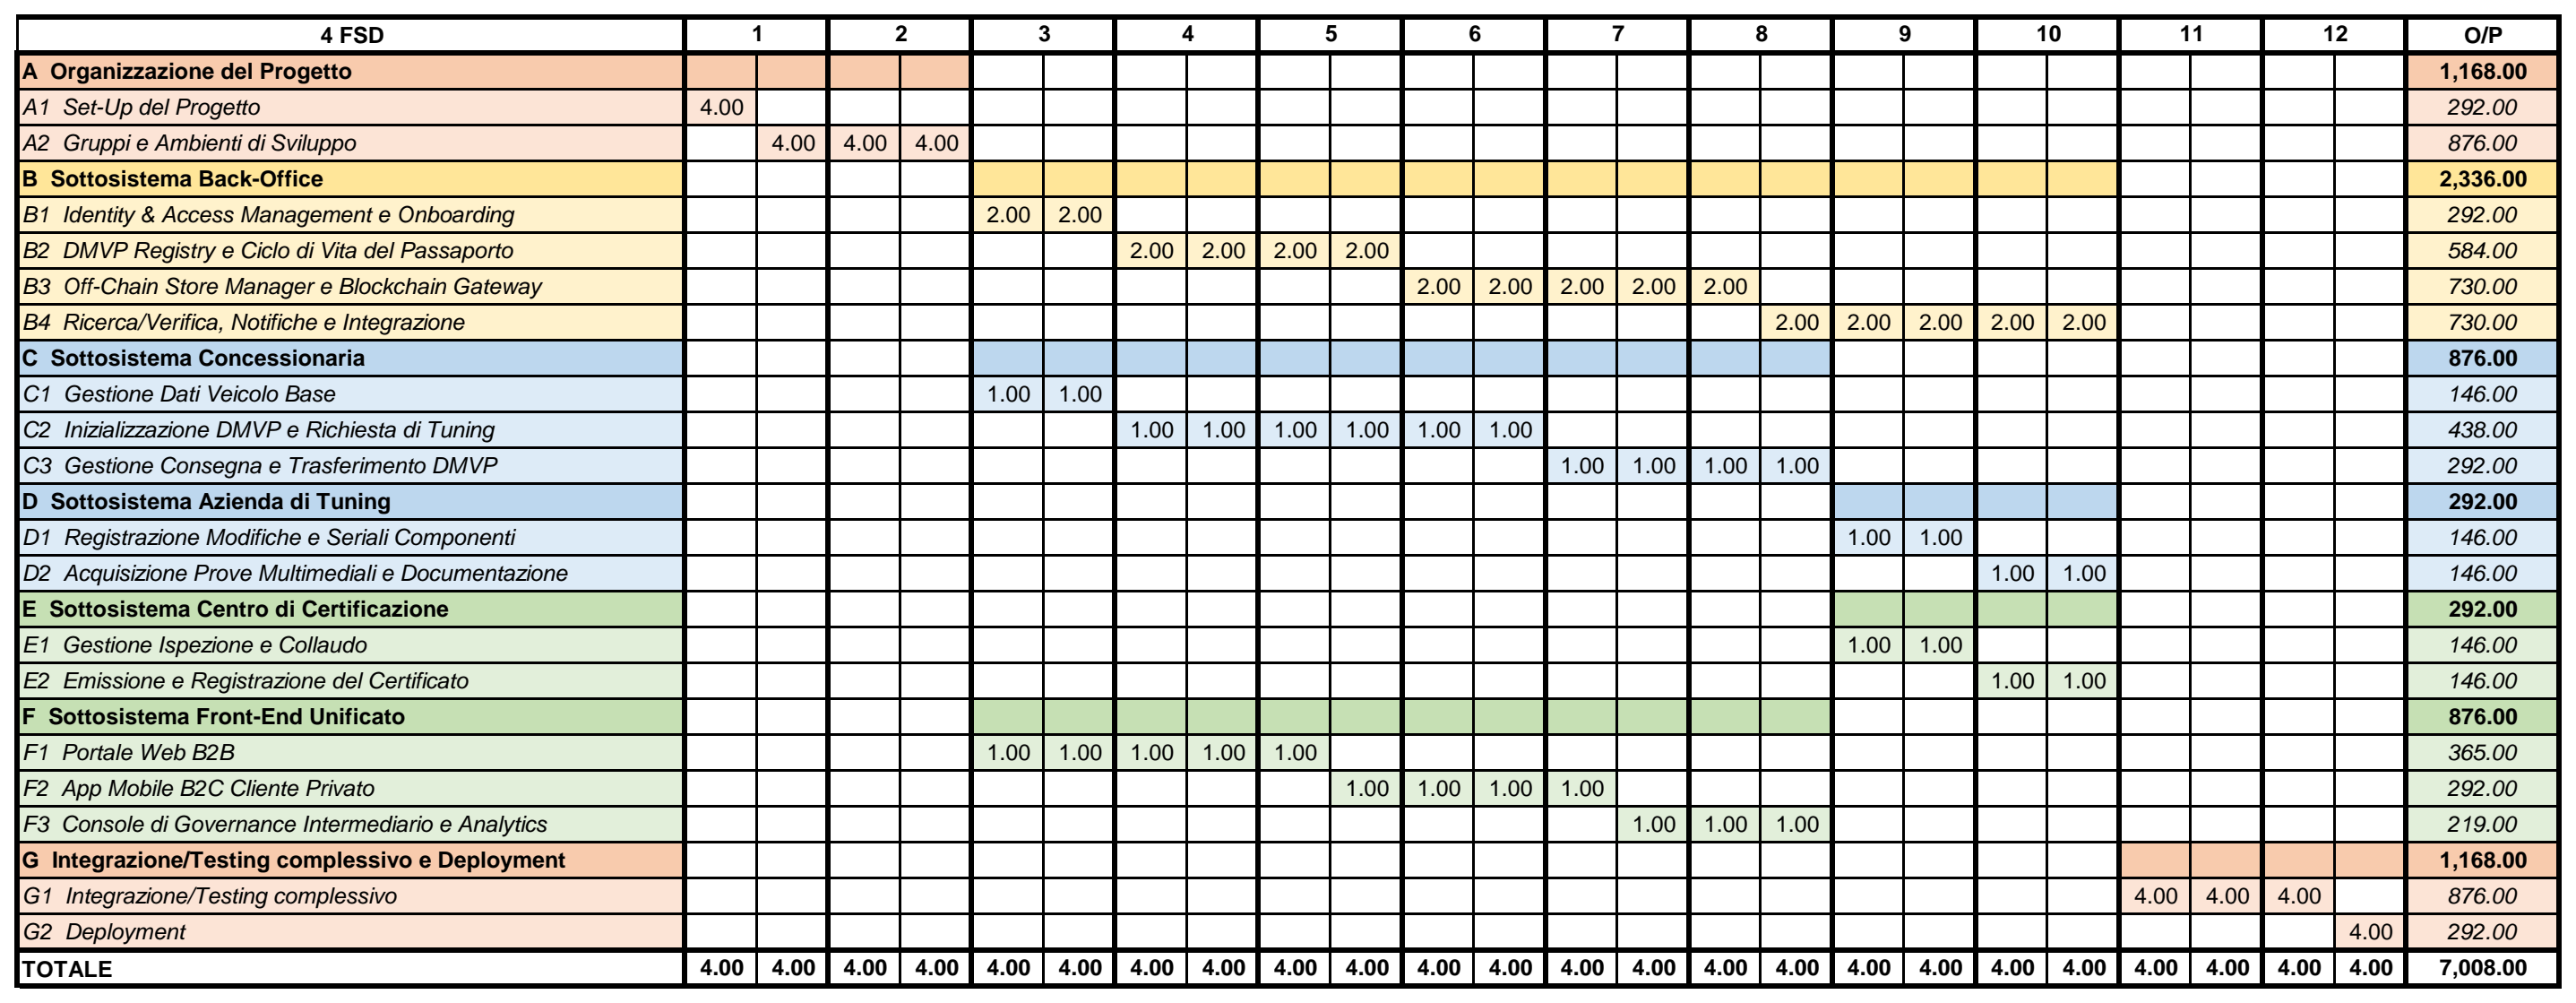
\includegraphics[width=\textwidth]{imgs/gantt/gantt_fase1/gantt_fase1_FSD.png}
    \caption{Impegno dei Full Stack Developer nella Fase 1}
    \label{fig:impegno-fsd-fase1}
\end{figure}
\begin{figure}[H]
    \centering
    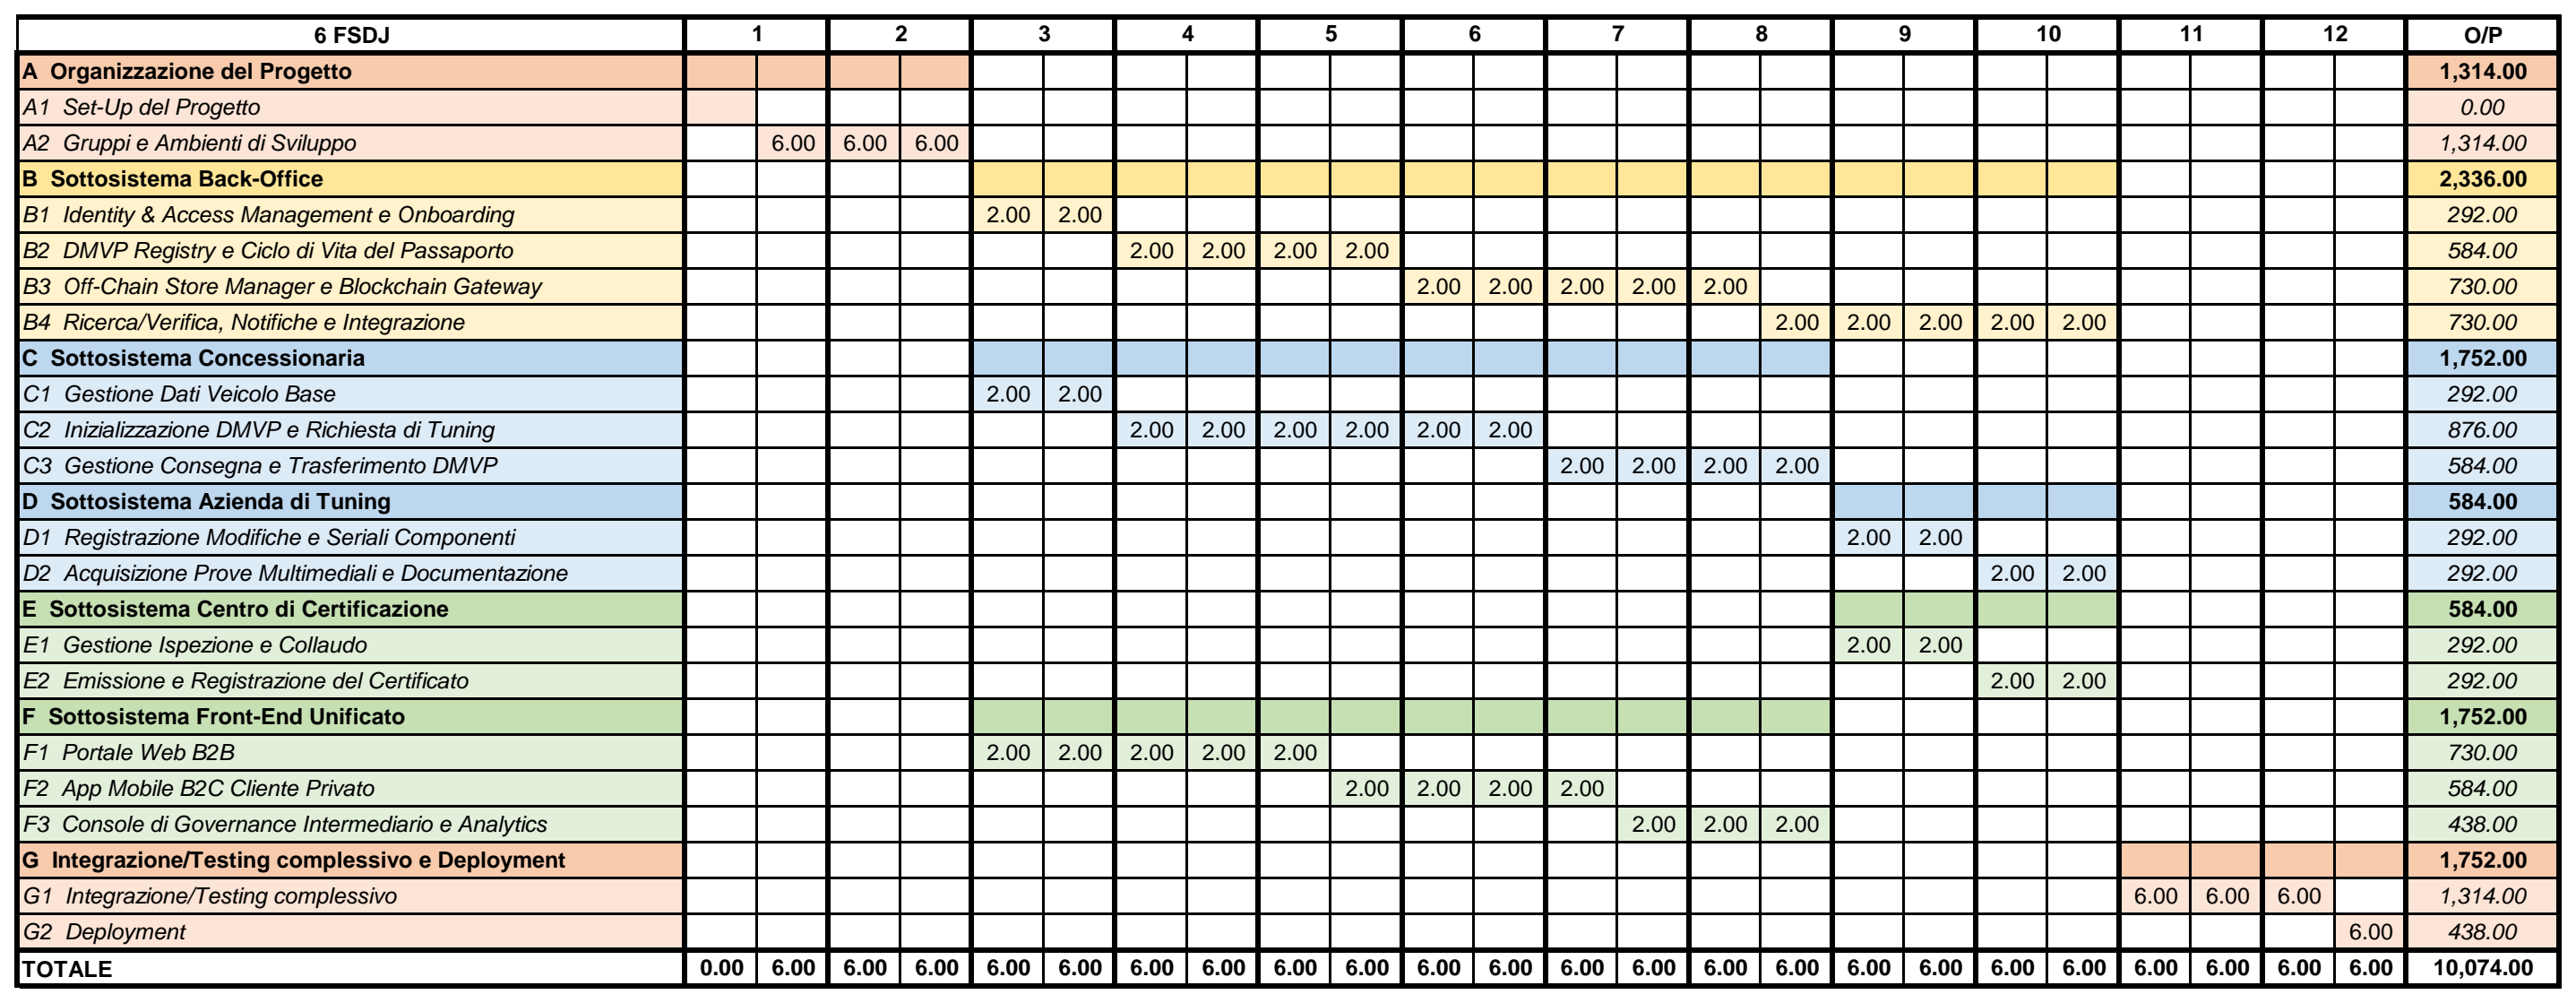
\includegraphics[width=\textwidth]{imgs/gantt/gantt_fase1/gantt_fase1_FSDJ.png}
    \caption{Impegno dei Full Stack Developer Junior nella Fase 1}
    \label{fig:impegno-fsdj-fase1}
\end{figure}
\begin{figure}[H]
    \centering
    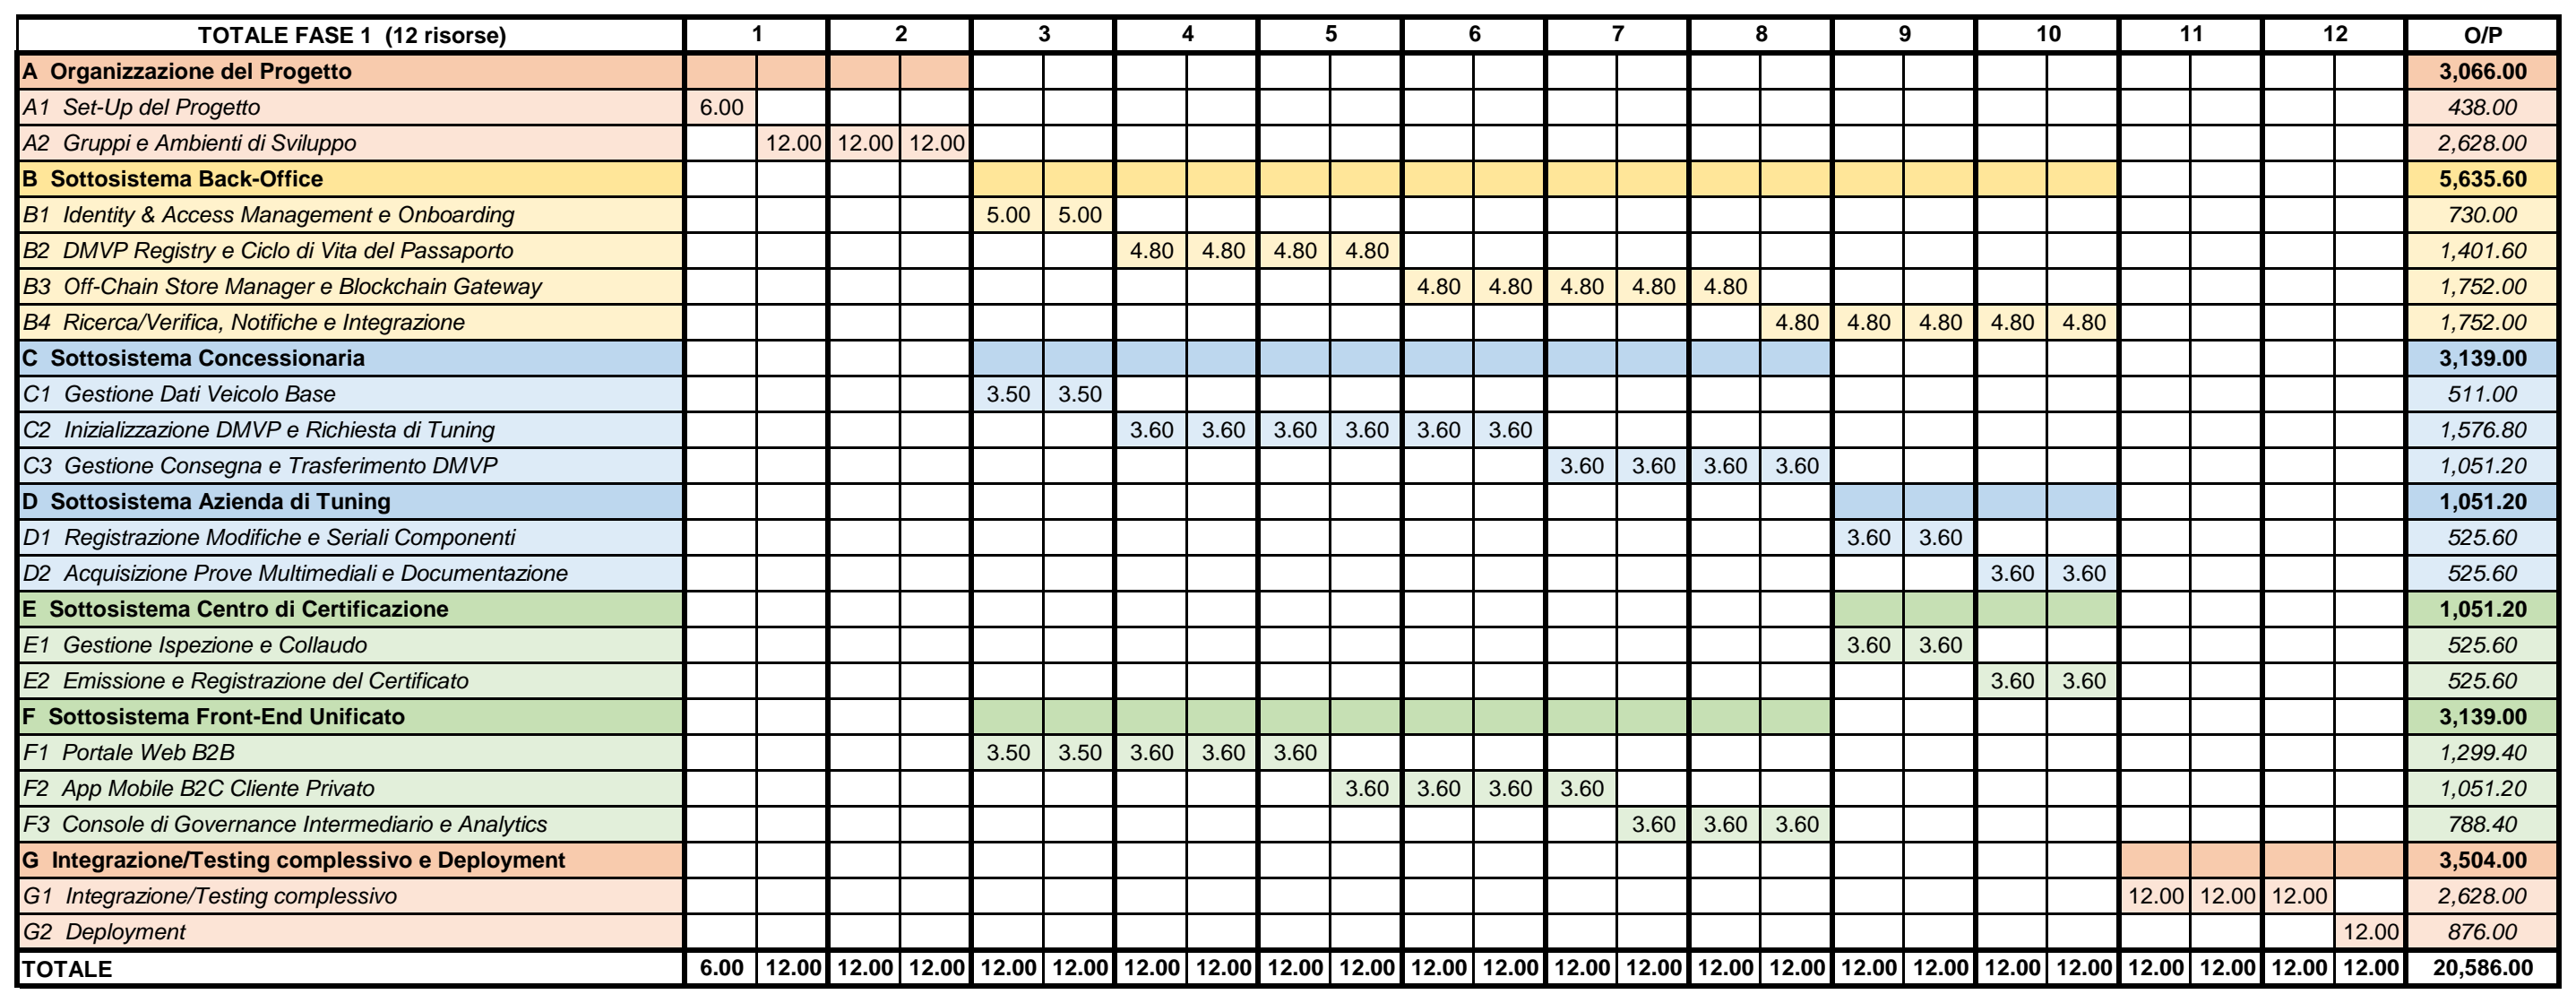
\includegraphics[width=\textwidth]{imgs/gantt/gantt_fase1/gantt_fase1_totale.png}
    \caption{Impegno totale delle risorse nella Fase 1}
    \label{fig:impegno-totale-fase1}
\end{figure}

\section{Pianificazione della Seconda Fase del Progetto: Esercizio della Piattaforma}

Successivamente alla pianificazione della prima fase, incentrata sullo sviluppo e sul rilascio della soluzione software, si rende necessaria la strutturazione della seconda fase del ciclo di vita del progetto, relativa al periodo di \textbf{esercizio, manutenzione e monitoraggio operativo} della piattaforma, su un orizzonte temporale di \textbf{cinque anni}.

Al fine di garantire la continuità operativa, l'integrità del registro distribuito e la progressiva espansione della rete, sono stati definiti cinque Task macro-funzionali, riassunti nella Tabella~\ref{tab:task-fase2}.

\begin{table}[H]
\centering
\small
\begin{tabular}{cp{4cm}p{7.5cm}}
\hline
\textbf{Cod.} & \textbf{Task} & \textbf{Descrizione} \\
\hline
A & Promozione della Piattaforma e Assistenza Commerciale & Campagne di marketing, presentazioni commerciali a concessionarie e reti di tuning, gestione delle trattative e personalizzazione dell'offerta. \\
B & Manutenzione Ordinaria & Aggiornamenti di sicurezza, correzione dei difetti, monitoraggio delle prestazioni e gestione dei nodi della rete permissioned. \\
C & Manutenzione Evolutiva & Nuove funzionalità in risposta alle esigenze degli utenti e alle evoluzioni normative; integrazione con nuovi sistemi esterni. \\
D & Assistenza e Onboarding degli Attori & Supporto tecnico e formazione di concessionarie, aziende di tuning e centri di certificazione; gestione delle identità di rete. \\
E & Analisi dei Dati di Esercizio & Raccolta e analisi dei dati d'uso, reportistica per gli attori business e supporto alle decisioni strategiche. \\
\hline
\end{tabular}
\caption{Task della Seconda Fase}
\label{tab:task-fase2}
\end{table}

La seconda fase non richiede l'impiego dell'intero organico iniziale, bensì prevede una contrazione strutturale del team per ottimizzare i costi di gestione. Il nucleo operativo viene ridotto da \textbf{12 a 8 risorse} complessive, riunite in un unico gruppo di gestione dell'esercizio (Figura~\ref{fig:gruppi-fase2}) così composto:

\begin{itemize}
    \item \textbf{0,5 Project Manager (PM)}, con funzioni di controllo di gestione e governance commerciale.
    \item \textbf{0,5 Software Architect (SA)}, incaricato della supervisione di alto livello dell'infrastruttura di rete.
    \item \textbf{2 Full Stack Developer (FSD)}, dedicati alla stabilità del back-end e dell'integrazione con la rete permissioned.
    \item \textbf{4 Full Stack Developer Junior (FSDJ)}, allocati sulle attività di assistenza e di aggiornamento delle interfacce.
\end{itemize}

\begin{figure}[H]
    \centering
    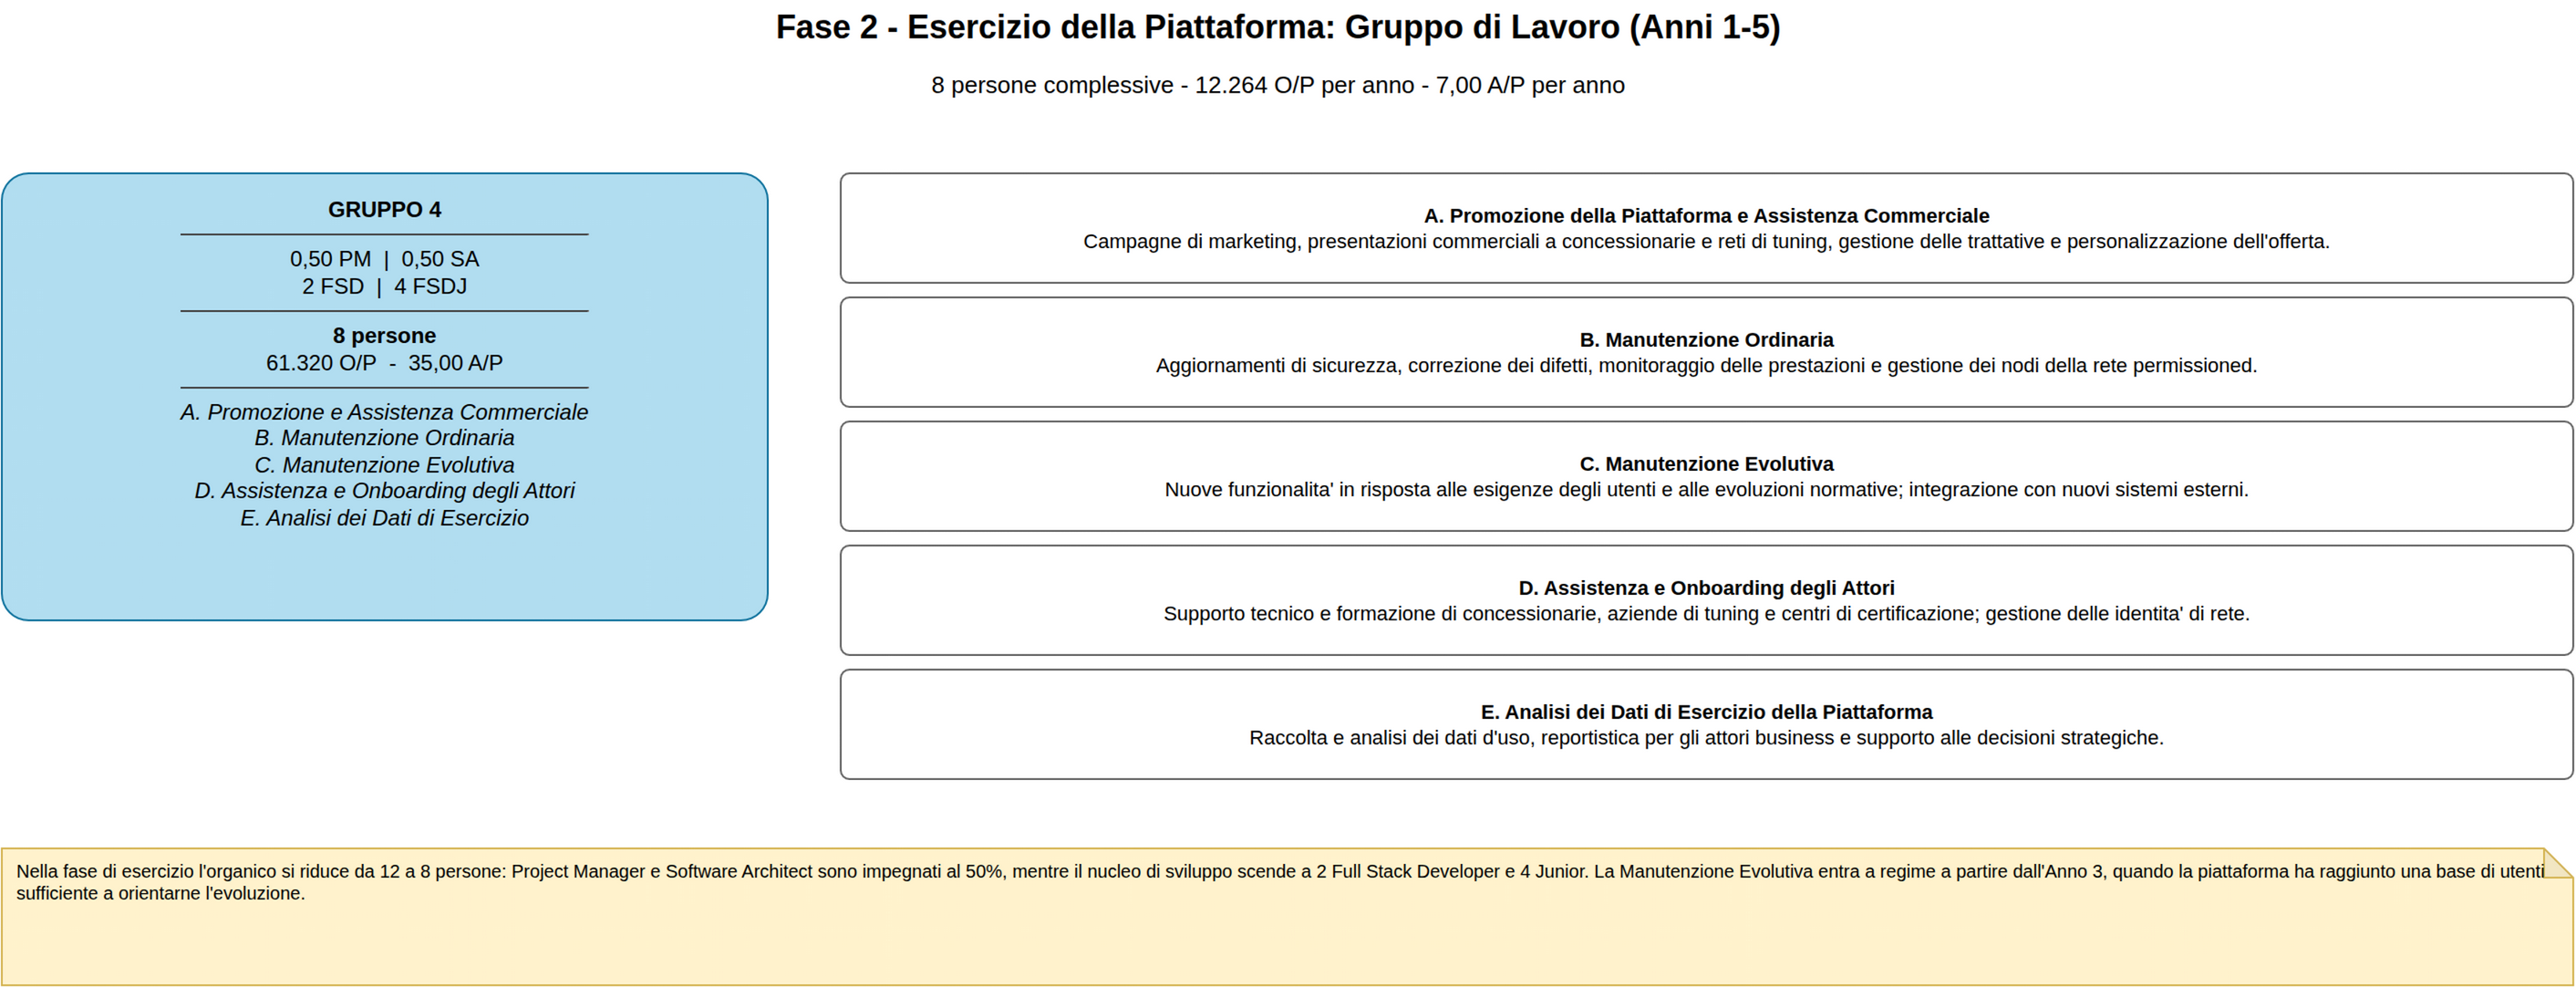
\includegraphics[width=\textwidth]{imgs/projectplan/09_gruppi_fase2.png}
    \caption{Gruppo di lavoro della Fase 2}
    \label{fig:gruppi-fase2}
\end{figure}

Il cronoprogramma delle attività per i cinque anni di esercizio prevede un impegno lineare e costante per l'\textbf{Analisi dei Dati di Esercizio}, che assorbe 1,55 A/P in ciascuno dei cinque anni, mentre gli altri task seguono un andamento articolato in due periodi distinti. Nei primi due anni le risorse si concentrano sulla \textbf{Manutenzione Ordinaria}, sull'\textbf{Assistenza e Onboarding degli Attori} e sulla \textbf{Promozione}, necessarie a stabilizzare la rete e ad acquisire i primi intermediari. A partire dall'\textbf{Anno 3} entra a regime la \textbf{Manutenzione Evolutiva}, quando la piattaforma ha raggiunto una base di utenti sufficiente a orientarne l'evoluzione: l'impegno su di essa (2,55 A/P) viene ricavato riducendo quello destinato agli altri tre task, la cui intensità si contrae una volta superata la fase di avviamento.

La ripartizione dell'impegno annuo tra i cinque Task \`e riportata nella Tabella~\ref{tab:op-fase2} e trova rappresentazione temporale nel diagramma di GANTT di Figura~\ref{fig:gantt-fase2}, articolato sui venti trimestri del quinquennio.

\begin{table}[H]
\centering
\small
\makebox[\textwidth][c]{%
\begin{tabular}{clrrrrrr}
\hline
\textbf{Cod.} & \textbf{Task} & \textbf{Anno 1} & \textbf{Anno 2} & \textbf{Anno 3} & \textbf{Anno 4} & \textbf{Anno 5} & \textbf{Totale} \\
\hline
A & Promozione e Assistenza Commerciale & 1.051,2 & 1.051,2 &   700,8 &   700,8 &   700,8 &  4.204,8 \\
B & Manutenzione Ordinaria                                & 5.080,8 & 5.080,8 & 2.277,6 & 2.277,6 & 2.277,6 & 16.994,4 \\
C & Manutenzione Evolutiva                                &       0 &       0 & 4.467,6 & 4.467,6 & 4.467,6 & 13.402,8 \\
D & Assistenza e Onboarding degli Attori                  & 3.416,4 & 3.416,4 & 2.102,4 & 2.102,4 & 2.102,4 & 13.140,0 \\
E & Analisi dei Dati di Esercizio & 2.715,6 & 2.715,6 & 2.715,6 & 2.715,6 & 2.715,6 & 13.578,0 \\
\hline
& \textbf{TOTALE O/P} & \textbf{12.264} & \textbf{12.264} & \textbf{12.264} & \textbf{12.264} & \textbf{12.264} & \textbf{61.320} \\
& \textbf{TOTALE A/P} & \textbf{7,00} & \textbf{7,00} & \textbf{7,00} & \textbf{7,00} & \textbf{7,00} & \textbf{35,00} \\
\hline
\end{tabular}}
\caption{Impegno annuo per Task della Seconda Fase (Ore-Persona)}
\label{tab:op-fase2}
\end{table}

\begin{figure}[H]
    \centering
    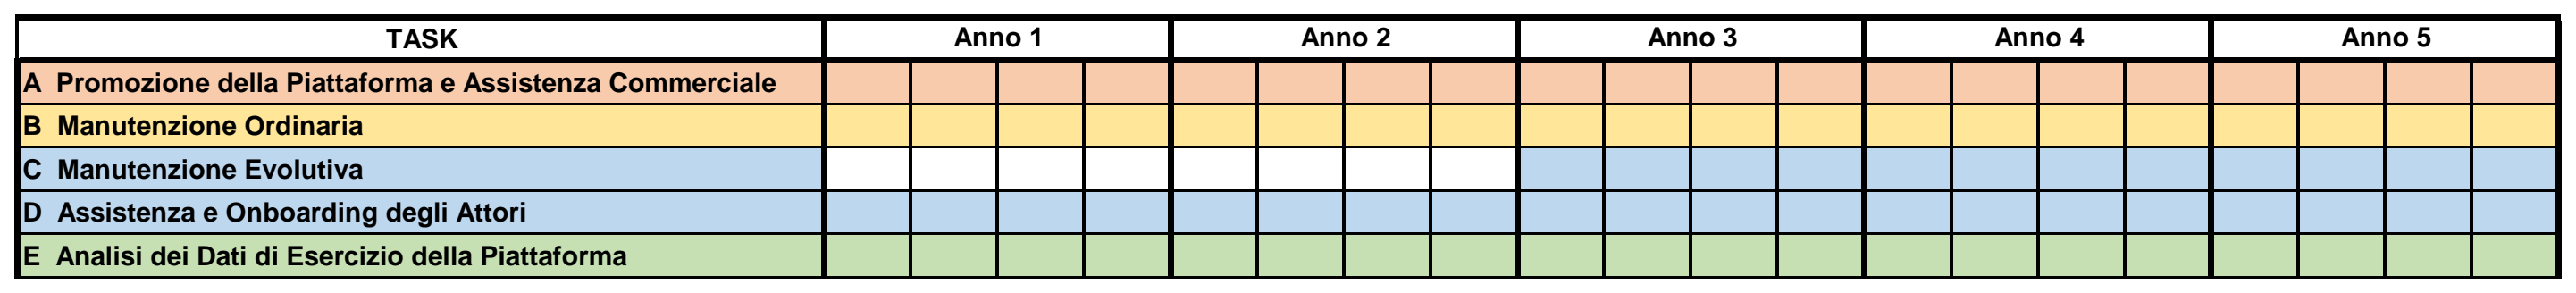
\includegraphics[width=\textwidth]{imgs/gantt/gantt_fase2/gantt_fase2.png}
    \caption{Diagramma di GANTT della Fase 2}
    \label{fig:gantt-fase2}
\end{figure}

L'impiego delle singole figure professionali nel corso del quinquennio di esercizio \`e riportato nei prospetti delle Figure~\ref{fig:impegno-pm-fase2}, \ref{fig:impegno-sa-fase2}, \ref{fig:impegno-fsd-fase2}, \ref{fig:impegno-fsdj-fase2} e~\ref{fig:impegno-totale-fase2}, costruiti con la medesima logica adottata per la Fase~1: l'unità temporale \`e in questo caso il trimestre, pari a 438 Ore-Persona per risorsa a tempo pieno, e il valore di ciascuna cella esprime il numero di risorse impegnate nel trimestre.

\begin{figure}[H]
    \centering
    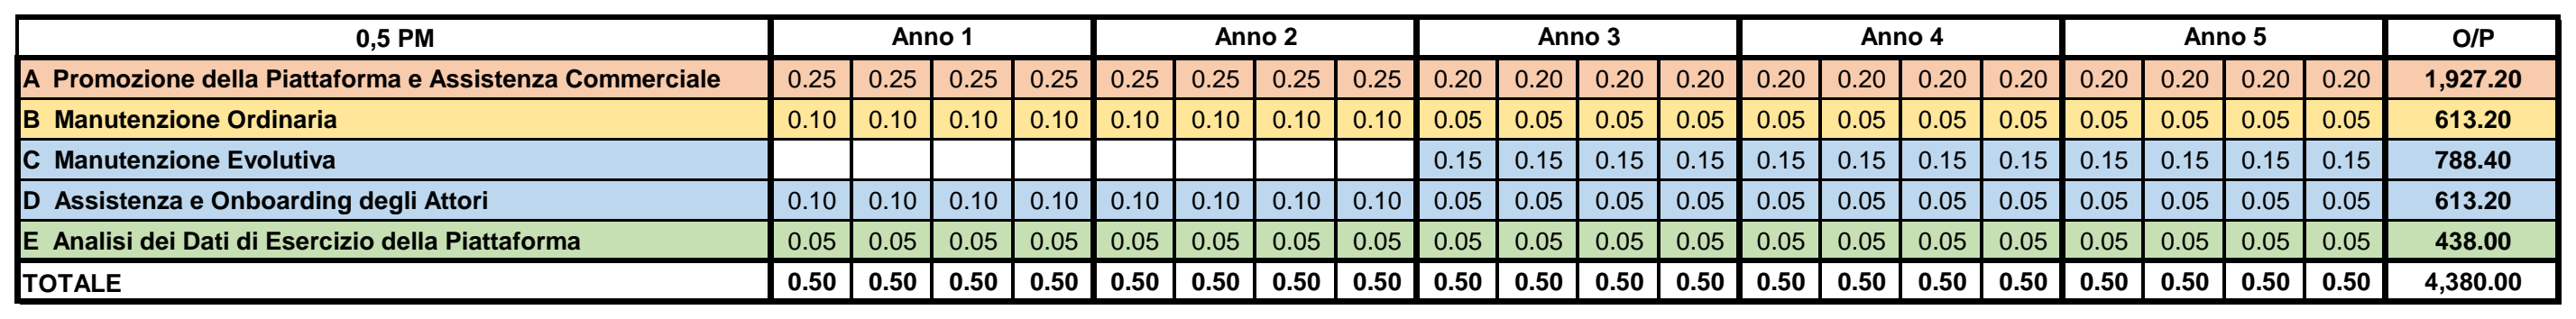
\includegraphics[width=\textwidth]{imgs/gantt/gantt_fase2/gantt_fase2_PM.png}
    \caption{Impegno del Project Manager nella Fase 2}
    \label{fig:impegno-pm-fase2}
\end{figure}
\begin{figure}[H]
    \centering
    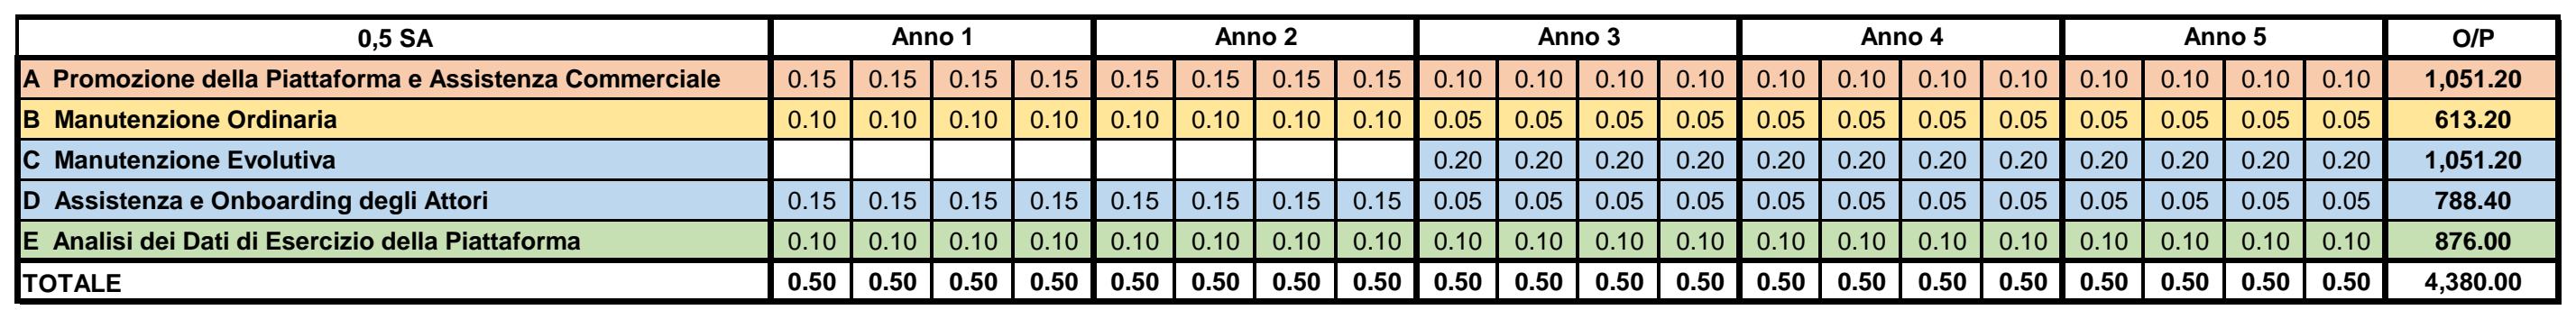
\includegraphics[width=\textwidth]{imgs/gantt/gantt_fase2/gantt_fase2_SA.png}
    \caption{Impegno del Software Architect nella Fase 2}
    \label{fig:impegno-sa-fase2}
\end{figure}
\begin{figure}[H]
    \centering
    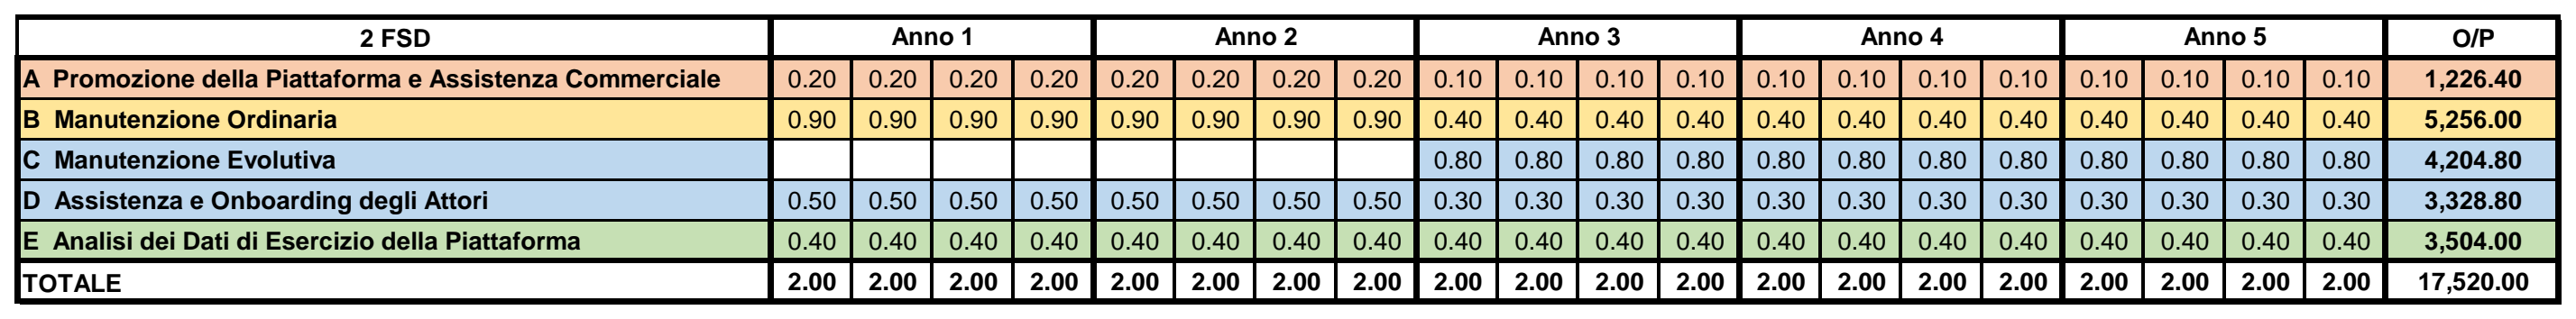
\includegraphics[width=\textwidth]{imgs/gantt/gantt_fase2/gantt_fase2_FSD.png}
    \caption{Impegno dei Full Stack Developer nella Fase 2}
    \label{fig:impegno-fsd-fase2}
\end{figure}
\begin{figure}[H]
    \centering
    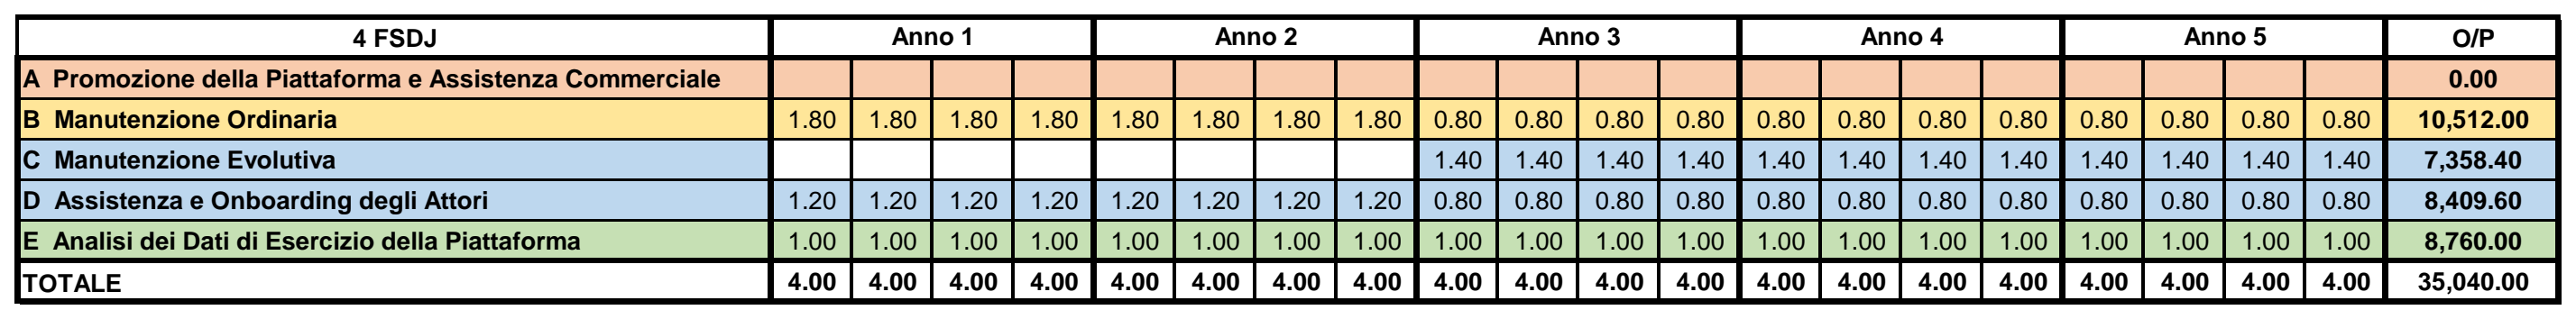
\includegraphics[width=\textwidth]{imgs/gantt/gantt_fase2/gantt_fase2_FSDJ.png}
    \caption{Impegno dei Full Stack Developer Junior nella Fase 2}
    \label{fig:impegno-fsdj-fase2}
\end{figure}
\begin{figure}[H]
    \centering
    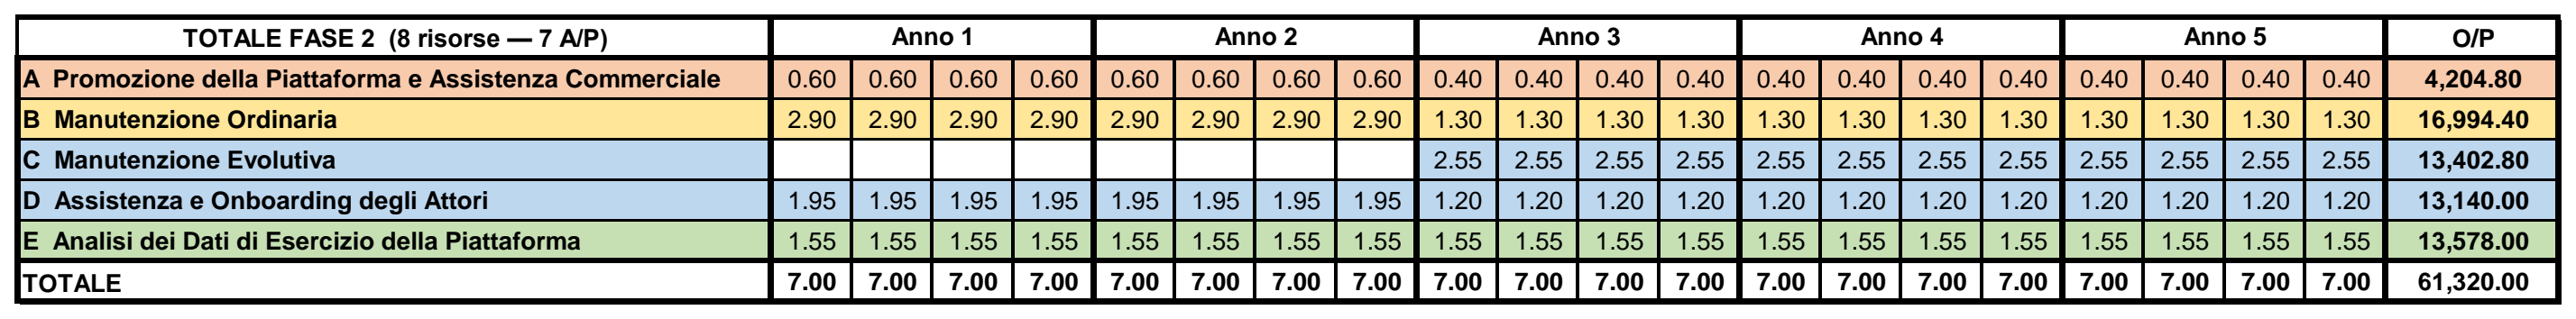
\includegraphics[width=\textwidth]{imgs/gantt/gantt_fase2/gantt_fase2_totale.png}
    \caption{Impegno totale delle risorse nella Fase 2}
    \label{fig:impegno-totale-fase2}
\end{figure}

\section{Riepilogo delle Risorse Umane Utilizzate}

A conclusione della pianificazione di progetto viene tracciato un quadro sinottico e comparativo dell'utilizzo delle risorse umane nel corso dei sei anni complessivi di ciclo di vita della piattaforma, evidenziando la transizione tra l'Anno 0 (Fase 1, sviluppo) e gli Anni 1--5 (Fase 2, esercizio).

L'impiego del personale, originariamente espresso in Ore-Persona (O/P), è riportato nella Tabella~\ref{tab:riepilogo-op} e successivamente convertito nell'unità di misura standard degli Anni-Persona (A/P) nella Tabella~\ref{tab:riepilogo-ap}, assumendo come parametro di riferimento un coefficiente di 1.752 ore lavorative annue per risorsa a tempo pieno.

\begin{table}[H]
\centering
\small
\makebox[\textwidth][c]{%
\begin{tabular}{lrrrrrrr}
\hline
\textbf{Figura} & \textbf{Anno 0} & \textbf{Anno 1} & \textbf{Anno 2} & \textbf{Anno 3} & \textbf{Anno 4} & \textbf{Anno 5} & \textbf{Totale} \\
\hline
PM   &  1.752 &    876 &    876 &    876 &    876 &    876 &  6.132 \\
SA   &  1.752 &    876 &    876 &    876 &    876 &    876 &  6.132 \\
FSD  &  7.008 &  3.504 &  3.504 &  3.504 &  3.504 &  3.504 & 24.528 \\
FSDJ & 10.074 &  7.008 &  7.008 &  7.008 &  7.008 &  7.008 & 45.114 \\
\hline
\textbf{TOTALE O/P} & \textbf{20.586} & \textbf{12.264} & \textbf{12.264} & \textbf{12.264} & \textbf{12.264} & \textbf{12.264} & \textbf{81.906} \\
\textbf{N.\ persone} & \textbf{12} & \textbf{8} & \textbf{8} & \textbf{8} & \textbf{8} & \textbf{8} & \\
\hline
\end{tabular}}
\caption{Impegno annuale del personale in Ore-Persona}
\label{tab:riepilogo-op}
\end{table}

\begin{table}[H]
\centering
\small
\makebox[\textwidth][c]{%
\begin{tabular}{lrrrrrrr}
\hline
\textbf{Figura} & \textbf{Anno 0} & \textbf{Anno 1} & \textbf{Anno 2} & \textbf{Anno 3} & \textbf{Anno 4} & \textbf{Anno 5} & \textbf{Totale} \\
\hline
PM   & 1,00 & 0,50 & 0,50 & 0,50 & 0,50 & 0,50 &  3,50 \\
SA   & 1,00 & 0,50 & 0,50 & 0,50 & 0,50 & 0,50 &  3,50 \\
FSD  & 4,00 & 2,00 & 2,00 & 2,00 & 2,00 & 2,00 & 14,00 \\
FSDJ & 5,75 & 4,00 & 4,00 & 4,00 & 4,00 & 4,00 & 25,75 \\
\hline
\textbf{TOTALE A/P} & \textbf{11,75} & \textbf{7,00} & \textbf{7,00} & \textbf{7,00} & \textbf{7,00} & \textbf{7,00} & \textbf{46,75} \\
\textbf{N.\ persone} & \textbf{12} & \textbf{8} & \textbf{8} & \textbf{8} & \textbf{8} & \textbf{8} & \\
\hline
\end{tabular}}
\caption{Impegno annuale del personale in Anni-Persona}
\label{tab:riepilogo-ap}
\end{table}

Come evidenziato dai dati, emerge una marcata differenziazione nel dimensionamento del personale in relazione alle specifiche sfide ingegneristiche di ciascun periodo:

\begin{enumerate}
    \item \textbf{Fase 1 (Sviluppo)}: richiede un team allargato e altamente specializzato, composto da \textbf{12 persone}. La forte concentrazione di sviluppatori (4 senior e 6 junior) si rende indispensabile per parallelizzare la costruzione dei cinque sottosistemi applicativi e della componente blockchain, minimizzando il \textit{Time-to-Market}.
    \item \textbf{Fase 2 (Esercizio)}: consente una contrazione del team a \textbf{8 persone}. Una volta effettuato il deployment e consolidato il chaincode sulla rete permissioned, le attività si spostano su compiti di monitoraggio, assistenza agli attori e rilascio di aggiornamenti incrementali, operazioni gestibili in piena sicurezza ed efficienza da un organico ridotto e ottimizzato.
\end{enumerate}

I valori di impegno riportati in questo capitolo costituiscono la base di calcolo per la stima dei costi del personale sviluppata nel Business Plan (Capitolo~7).